

\chapter*{Notational Conventions and Preliminaries}
\addcontentsline{toc}{chapter}{Notational Conventions and Preliminaries}

\label{ch0-conventions}
\section{Some abbreviations frequently
used throughout this book}

\begin{itemize}
\item
bnet= Bnet= Bayesian Network
\item
CPT = Conditional Probabilities Table,
 same as TPM
\item
DAG = Directed Acyclic Graph
\item
i.i.d.= independent identically
distributed.
 \item
 RCT= Randomized Controlled Trial,
a.k.a. A/B testing.

\item
TPM= Transition Probability Matrix,
same as CPT

\end{itemize}

\section{${\cal N}(!a)$}
$\caln(!a)$ will denote
a normalization constant that does not depend
on $a$. For example, $P(x)=\caln(!x)e^{-x}$
where $\int_0^\infty dx \;P(x)=1$.

\section{One hot vector}
A {\bf one hot  vector}
is a vector with all entries
equal to zero with
the exception of a single entry which is one.
A {\bf one cold vector}  is a vector with all entries
equal to one with the exception of  a
single entry which is zero.
For example, if $x^n=(x_0, x_1, \ldots,
x_{n-1})$ and
$x_i=\delta(i,0)$ then $x^n$ is one hot.

Two types of
sets that one frequently encounters
are {\bf categorical sets} (a.k.a. ``nominal sets", i.e.,
sets with ``named" elements, with elements given a ``nomme")
and {\bf numerical sets} (a.k.a. ``ordinal sets", i.e., sets
 with ``ordered"
elements).
For example, $\{1,2,5\}$ is a numerical set
because its elements have a natural order,
and $\{\text{cat, dog, bird}\}$ is a  categorical set
because its elements don't have a natural order.

In Machine Learning (ML),
one often encodes categorical sets as one-hot vectors.
For example, suppose we have 4 binary registers (i.e., nodes)
 $x_3, x_2,x_1, x_0$
and  the categorical set $\{\text{cat, dog, canary}\}$.
Then a possible {\bf one-hot encoding}
of the set
is cat=0001, dog=0010 and canary=0100.
This differs from
a {\bf binary encoding} of the set such as
cat=0000, dog=0001, canary=0011.
Clearly, a binary encoding requires
fewer registers than a one-hot
encoding to
encode the same set,
and the one-hot encoding
of a set with $n$ elements requires
$n$ or more registers.

\section{Special sets}
Define $\ZZ, \RR, \CC$ to be
 the integers, real numbers
 and complex numbers, respectively.

For $a<b$, define $\ZZ_I$
to be the integers in the
interval $I$, where
$I=[a,b],[a,b),(a,b],(a,b)$
(i.e, $I$ can be closed or
 open on either side).

$A_{>0}=\{k\in A: k>0\}$ for $A=\ZZ, \RR$.

\section{Kronecker
delta function}

 For $x,y$ in discrete set $S$,
\beq
\delta(x,y)=\left\{
\begin{array}{l}
1\;{\rm if}\; x=y
\\
0 \;{\rm if}\; x\neq y
\end{array}
\right.
\eeq

\section{Dirac delta function}
 For $x,y\in\RR$,
\beq
\int^{+\infty}_{-\infty}dx\;\delta(x-y)f(x)=f(y)
\eeq

\section{Indicator function
(a.k.a. Truth function)}
\beq
\indi(\cals)=\left\{
\begin{array}{l}
1\;{\rm if\; \cals\; is\; true}
\\
0 \;{\rm if \;\cals\; is \;false}
\end{array}
\right.
\eeq
For example, $\delta(x,y)=\indi(x=y)$.

\section{Majority function}
The {\bf majority function}  is defined as follows.

\beq
\begin{array}{ll}
{\tt majority}(L)=&
\text{ most common element of  list $L$}
\\
&\text{(ties resolved by chance)}
\end{array}
\eeq
Note that the majority function
acts on lists, not sets. By definition,
all elements of a set appear only once in the set.
${\tt majority}(L)$
is usually
used when the elements of
$L$ are categorical (i.e., not real numbers).
When they are real numbers,
it makes more sense to use, instead of
${\tt majority}(L)$, a simple average
of the elements of $L$.


\section{Underlined letters
 indicate random variables}
Random variables will be indicated by
underlined letters and their values
by non-underlined letters.
 Each node of a bnet will be
 labelled by a random variable.
 Thus, $\rvx=x$ means that node
$\rvx$ is in state $x$.

It is more
conventional to
use an upper
case letter to
indicate
a random
variable
and a lower case letter
for its state.
Thus, $X=x$ means that
random variable
$X$ is in state $x$.
However,
we have
opted
in this
book to
avoid
that notation,
because
we often
want to define
certain lower
case letters
to be random variables
or, conversely, define certain upper
case letters to
be non-random variables.

\section{Probability distributions}
 $P_\rvx(x)=P(\rvx=x)=P(x)$ is the probability that random variable $\rvx$ equals $x\in S_\rvx$. $S_\rvx$ is the set of states (i.e., values) that $\rvx$ can assume and $n_\rvx = |S_\rvx|$ is the size (a.k.a. cardinality) of that set. Hence,
\beq
\sum_{x\in S_\rvx}P_\rvx(x)=1
\eeq

\hrule
\beq
P_{\rvx,\rvy}(x,y)=P(\rvx=x, \rvy=y)=P(x,y)
\eeq
\beq
P_{\rvx|\rvy}(x|y)=P(\rvx=x| \rvy=y)=P(x|y)=\frac{P(x,y)}{P(y)}
\eeq



\section{Discretization
of continuous
probability distributions}

The TPM of a node
of a bnet can be either a discrete or
a continuous probability distribution.
To go from continuous to discrete, one
replaces integrals over states of a node
 by sums over new states, and Dirac delta
functions by Kronecker delta functions.
 More precisely, consider a function
$f: [a, b]\rarrow \RR$. Express
 $[a,b]$ as
a union of
small, disjoint (except for
one point) closed sub-intervals (bins) of
length $\Delta x$.
Name one point
in each bin to be the representative of that bin,
and  let $S_\rvx$ be the
set of all the bin representatives. This is called
discretization or binning. Then

\beq
\frac{1}{(b-a)}
\int_{[a,b]} dx \; f(x)\rarrow
\frac{\Delta x}{(b-a)} \sum_{x\in S_\rvx}f(x)
=
\frac{1}{n_\rvx} \sum_{x\in S_\rvx}f(x)
 \;.
\eeq
Both sides of last equation are 1 when $f(x)=1$.
 Furthermore, if $y\in S_\rvx$, then

\beq
\int_{[a,b]} dx \; \delta(x-y)f(x)=f(y)
\rarrow \sum_{x\in S_\rvx}\delta(x,y)f(x)
=f(y)
\;.
\eeq
\section{Samples,
i.i.d. variables}
\beq
\vec{x}= (x[0], x[1], x[2] \ldots,
 x[nsam(\vecx)-1])=x[:]
\eeq

 $nsam(\vecx)$ is the number of samples
 of $\vecx$.
$\rvx[\sigma]\in S_\rvx$ are
 i.i.d. (independent identically distributed)
samples with

 \beq
x[\sigma]\sim P_\rvx\;\;({\rm i.e.}\; P_{\ul{x[\sigma]}}=P_\rvx)
\eeq

\beq
P(\rvx=x)=\frac{1}{nsam(\vecx)}\sum_\sigma \indi(x[\sigma]=x)
\eeq
Hence, for any $f:S_\rvx\rarrow \RR$,
\beq
\sum_x P(\rvx=x)f(x)
=\frac{1}{nsam(\vecx)}\sum_\sigma f(x[\sigma])
\eeq


If we use two sampled variables, say $\vecx$ and $\vecy$,
in a given bnet, their number of samples
$nsam(\vecx)$ and $nsam(\vecy)$ need not be equal.

\hrule
\beq
P(\vecx) = \prod_\sigma P(x[\sigma])
\eeq

\beq
\sum_\vecx = \prod_\sigma\sum_{x[\sigma]}
\eeq

\beq
\partial_\vecx =
[\partial_{x[0]}, \partial_{x[1]},\partial_{x[2]}, \dots, \partial_{x[nsam(\vecx)-1]}]
\eeq

\hrule
\beqa
P(\vecx)&\approx& [\prod_x P(x)^{P(x)}]^{nsam(\vecx)} \\
&=& e^{nsam(\vecx)\sum_x P(x)\ln P(x)}\\
&=& e^{-nsam(\vecx)H(P_\rvx)}
\eeqa

\section{Expected Value and Variance}

Given a random variable
 $\rvx$ with states $S_\rvx$ and
a function $f:S_\rvx\rarrow \RR$, define

\beq
E_\rvx[f(\rvx)]=
E_{x\sim P(x)}[f(x)] = \sum_x P(x) f(x)
\eeq

\beqa
Var_\rvx[f(\rvx)]&=& E_\rvx
\left[(f(\rvx)-E_\rvx[f(\rvx)])^2\right]
\\
&=&
E_\rvx[f(\rvx)^2]-(E_\rvx[f(\rvx)])^2
\eeqa

\beq
E[\rvx]=E_\rvx[\rvx]
\eeq

\beq
Var[\rvx]=
Var_\rvx[\rvx]
\eeq



\section{Conditional Expected Value}

Given a random variable $\rvx$ with states $S_\rvx$, a random variable $\rvy$ with states $S_\rvy,$ and a function $f:S_\rvx\times S_\rvy\rarrow \RR$, define

\beq
E_{\rvx|\rvy}[f(\rvx, \rvy)]=
\sum_x P(x|\rvy) f(x, \rvy)
\;,
\eeq

\beq
E_{\rvx|\rvy=y}[f(\rvx, y)]=
E_{\rvx|y}[f(\rvx, y)]= \sum_x P(x| y) f(x, y)
\;.
\eeq
Note that

\beqa
E_\rvy[E_{\rvx|\rvy}[f(\rvx, \rvy)]]&=&
\sum_{x,y}P(x|y)P(y)f(x,y)
\\&=&
\sum_{x,y}P(x,y)f(x,y)
\\&=&
E_{\rvx, \rvy}[f(\rvx, \rvy)]
\;.
\eeqa



\section{Notation
for covariances}
Consider two random variables $\rvx, \rvy$.

\begin{itemize}
\item
Mean value of $\rvx$
\beq
\av{\rvx}=
E_\rvx[\rvx]
\eeq

\item
Signed distance of $\rvx$ to its mean value
\beq
\Delta \rvx = \rvx - \av{\rvx}
\eeq

\item
Covariance of $(\rvx, \rvy)$
\beq
Cov(\rvx, \rvy)=\av{\rvx, \rvy}=
\av{\Delta \rvx \Delta \rvy}
=
\av{\rvx\rvy}-\av{\rvx}\av{\rvy}
\eeq

$\av{\rvx, \rvy}$ is symmetric
(i.e., $\av{\rvx, \rvy}=\av{\rvy, \rvx}$)
and bilinear (i.e.,
$\av{\sum_i \alp_i\rvx_i, \rvy}
=
\sum_i\alp_i\av{\rvx_i, \rvy}$, where
$\alp_i\in \RR$
are non-random scalars
and $\rvx_i, \rvy\in\RR$ are
real-valued random
variables.)

\item
Variance of $\rvx$
\beq
Var(\rvx)=\av{\rvx, \rvx}
\eeq

\item
Standard deviation or $\rvx$
\beq
\sigma_\rvx=\sqrt{\av{\rvx, \rvx}}
\eeq

\item
Correlation Coefficient of $(\rvx, \rvy)$
\beq
\rho_{\rvx, \rvy}=
\frac{\av{\rvx, \rvy}}
{\sqrt{\av{\rvx, \rvx}\av{\rvy, \rvy}}}
\eeq
\end{itemize}

\section{Conditional Covariance}
Let $\rvx, \rvy, \rva$
be random variables.
The covariance $Cov(\rvx, \rvy|\rva)$
of $\rvx$ and $\rvy$
given $\rva$, is defined
the same
way as $Cov(\rvx, \rvy)$,
except that all
expected values are
conditioned on $\rva$.



\beq
Cov(\rvx, \rvy|\rva)=
\av{\rvx, \rvy}_{|\rva}
=
\av{(\rvx-\av{\rvx}_{|\rva})
(\rvy-\av{\rvy}_{|\rva})}_{|\rva}
\eeq
where

\beq
\av{\rvx}_{|\rva}=E_{\rvx|\rva}[\rvx]
\;.
\eeq

\section{Law of Total Variance}

\begin{claim}
Suppose $P:S_\rvx\times S_\rvy\rarrow [0,1]$
is a probability distribution.
Suppose $f:S_\rvx\times S_\rvy\rarrow \RR$
 and $f=f(x,y)$. Then
\beq
Var_{\rvx, \rvy}(f)=
E_\rvy[Var_{\rvx|\rvy}(f)]
+
Var_\rvy(E_{\rvx|\rvy}[f])
\;.
\eeq
In particular,
\beq
Var_{\rvx}(x)=
E_\rvy[Var_{\rvx|\rvy}(x)]
+
Var_\rvy(E_{\rvx|\rvy}[x])
\;.
\eeq

\end{claim}
\proof

Let
\beq
A=\sum_y P(y)\left(\sum_x P(x|y)f\right)^2
\;.
\eeq
Then

\beqa
Var_{\rvx, \rvy}(f)&=& \sum_{x,y}P(x,y)f^2 -
\left( \sum_{x,y} P(x,y) f\right)^2
\\
&=&
\left\{
\begin{array}{l}
\sum_{x,y}P(x,y)f^2
-A
\\
+\left(A-\left( \sum_{x,y} P(x,y) f\right)^2\right)
\end{array}
\right.
\eeqa

\beqa
E_\rvy[Var_{\rvx|\rvy}(f)]
&=&
\sum_y P(y)\left(\sum_x P(x|y)f^2
-
\left(\sum_x P(x|y)f\right)^2
\right)
\\
&=&
\sum_{x,y}P(x,y)f^2
-A
\eeqa

\beqa
Var_\rvy(E_{\rvx|\rvy}[f])
&=&
\sum_y P(y)
\left(\sum_x P(x|y)f\right)^2
-\left(
\sum_y P(y)\sum_xP(x|y)f
\right)^2
\\
&=&
A-\left( \sum_{x,y} P(x,y) f\right)^2
\eeqa
\qed





\section{Normal Distribution}


For $x, \mu, \sigma\in \RR$,
$\sigma >0$, we define the Normal Distribution
(see Fig.\ref{fig-norm-dist}) by

\beq
\caln(x; \mu, \sigma^2)=
\frac{1}{\sigma\sqrt{2\pi}}
e^{-\frac{1}{2}\left(
\frac{x-\mu}{\sigma}\right)^2}
\;.
\eeq

For a {\bf standard deviation}
$\s$, the {\bf precision} $\tau$
is defined as $\tau=\frac{1}{\s^2}$.

\begin{claim}
If

\beq
\rvx_1\sim \caln(\mu_1, \s^2_1)
\eeq
and

\beq
\rvx_2\sim \caln( \mu_2, \s^2_2)
\eeq
then
\beq
\rvx=\rvx_1 +\rvx_2 \sim \caln(\mu_1 + \mu_2, \s^2_1 + \s^2_2)
\;.
\eeq
\end{claim}
\proof

\beqa
P(\rvx=x)&=&\caln(!x)
\int_{-\infty}^{+\infty}dx_2\;
P(\rvx_1 + \rvx_2 = x|\rvx_2=x_2)P(x_2)
\\
&=&\caln(!x)
\int_{-\infty}^{+\infty}dx_2\;
\caln(x-x_2;\mu_1, \s^2_1)
\caln(x_2;\mu_2, \s^2_2)
\\
&=&
\caln(x;\mu_1 +\mu_2; \s^2_1+\s^2_2)
\eeqa
\qed

\begin{figure}[h!]
\centering
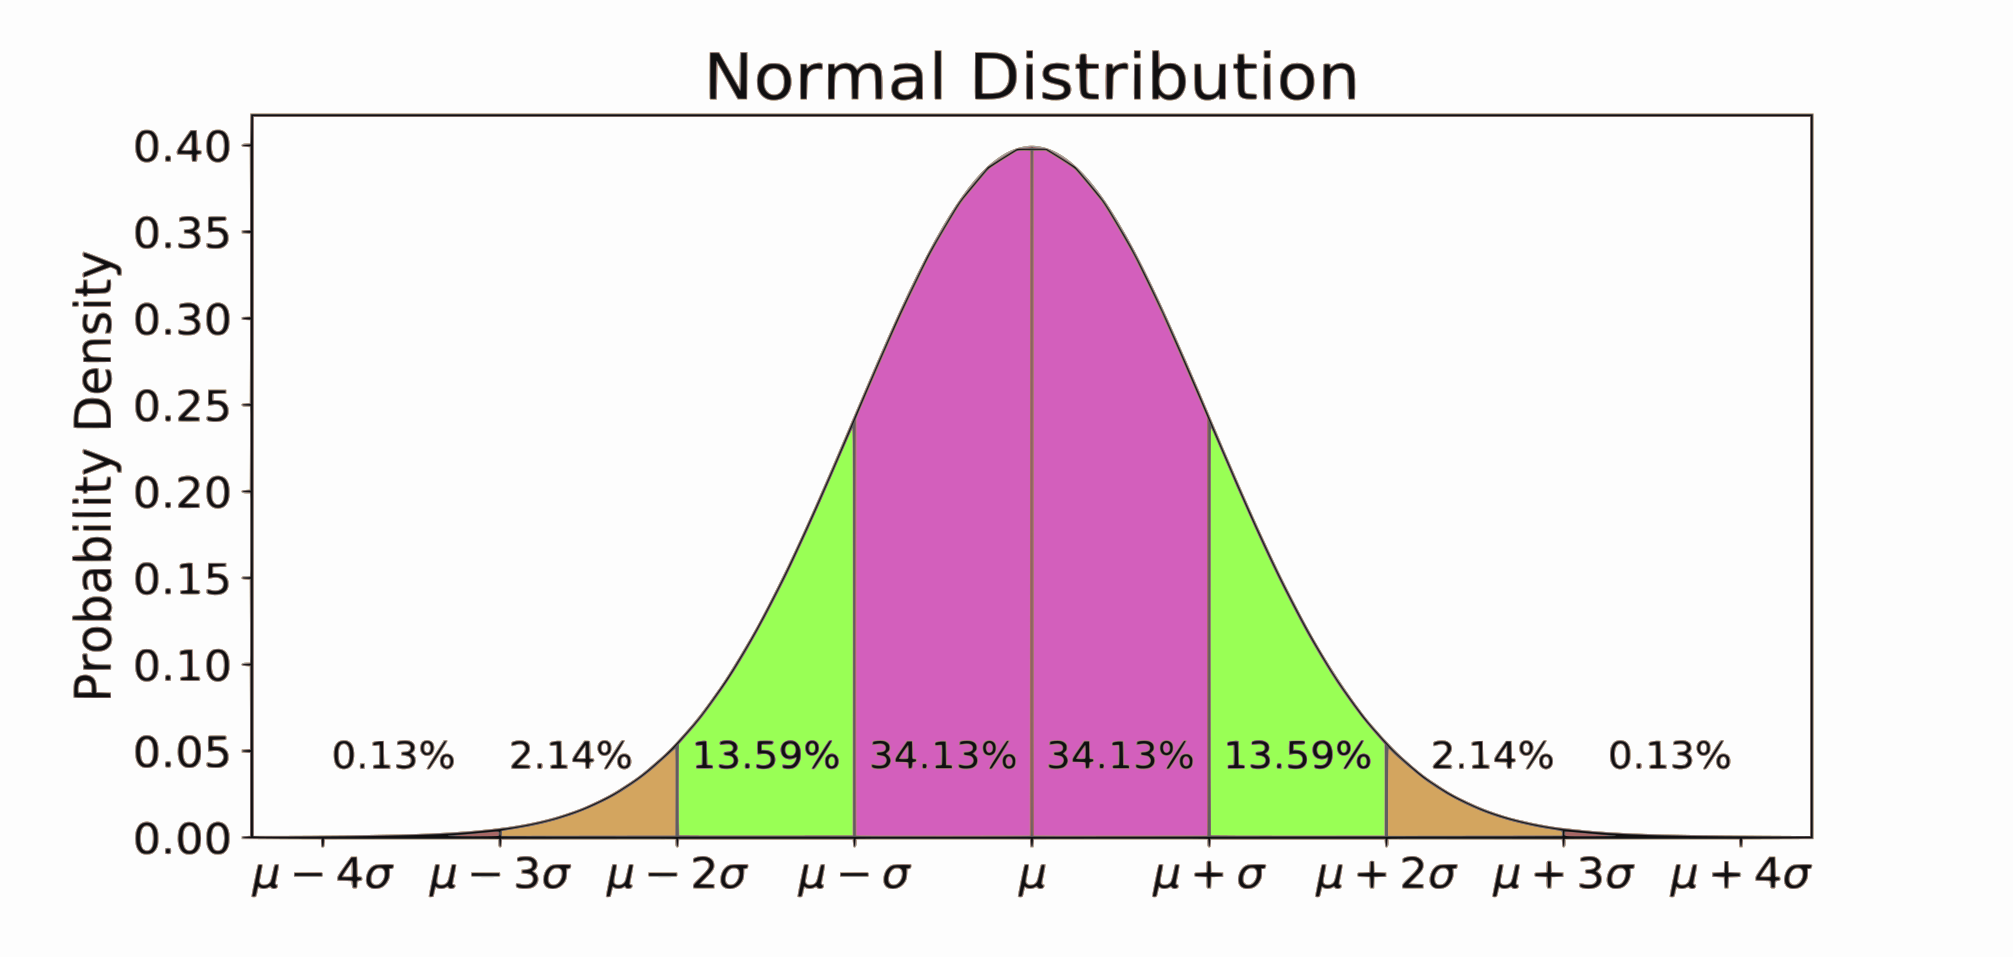
\includegraphics[width=5in]
{conventions/normal-dist.png}
\caption{Normal Distribution
$\caln(x;\mu, \s^2)$.}
\label{fig-norm-dist}
\end{figure}

The {\bf Standard Normal Distribution} $P_{SND}(x)$
and its cumulative distribution $\Phi(x)$ are defined by

\beq
P_{SND}(x)=\caln(x; \mu=0, \s=1)
\eeq

\beq
\Phi(x) = \int_{-\infty}^x dx'\;P_{SND}(x')
\eeq

The {\bf error function} ${\rm erf}:\RR\rarrow [-1,1]$
is defined by
\beq
{\rm erf}(x) = \frac{2}{\sqrt{\pi}}
\int_0^x du \; e^{-\frac{u^2}{2}}
\eeq

Note that

\beq
\Phi(x)= \frac{1}{2} + \frac{1}{2}{\rm erf}(x)
\label{eq-Phi-erf}
\eeq
Eq.(\ref{eq-Phi-erf})
is interpreted geometrically in Fig.\ref{fig-erf}.

\begin{figure}[h!]
\centering
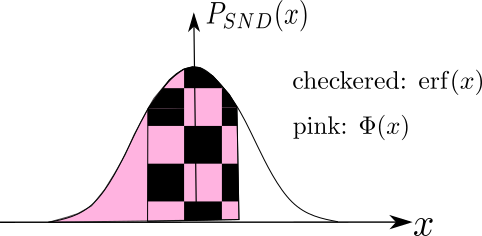
\includegraphics[width=2.8in]
{conventions/erf.png}
\caption{Plot of Standard
Normal Distribution $P_{SND}(x)$.
 Values of ${\rm erf}(x)$ and $\Phi(x)$
 equal indicated areas.}
 \label{fig-erf}
\end{figure}
\section{Uniform Distribution}
For $a<b$, $x\in [a,b]$

\beq
\calu(x;a,b) =
\frac{1}{b-a}
\eeq

\section {Softmax function
(a.k.a. Boltzmann Distribution)}

The Softmax function
 is defined by
\beq
P(x_i
|x.)=\frac{e^{x_i}}{\sum_i e^{x_i}}=
\softmax(x.)_i
\label{eq-softmax}
\eeq
The
Boltzmann distribution is defined as

\beq
P(\rvE_a=E_a)=\frac{\exp(-\frac{E_a}{kT})}{\sum_{a}
\exp(-\frac{E_{a}}{kT})}=
P(\frac{-E_a}{kT}|E.)\eeq
for a system with energies $E_a$
and temperature $T$,
where $k$
is Boltzmann's constant.

The function
softmax() is called softmax because if we
approximate the exponentials,
 both in the numerator and denominator
of Eq.(\ref{eq-softmax}),
by the largest one
of them or zero,
we get

\beq
\softmax(x.)_i\approx \indi(i=\argmax_k x_k)
\;.
\eeq
Thus, softmax($x.$)
returns a continuous
function that approximates a one-hot vector
that is 1 at the
$i$th
component, where
$i=\argmax_k(x_k)$,
and zero at the other components.

Note that
\beq
\pder{\ln P(x_i|x)}{x_a}
=
\pder{}{x_a}\ln\left[
\frac{e^{x_i}}{\sum_i e^{x_i}}
\right]
=
\delta(a,i)
-
P(x_a|x)
\eeq

For 2 variables $x_0, x_1$,
\beqa
P(x_0|x.)&=&
\frac{e^{x_0}}{e^{x_0} + e^{x_1}}\\
&=&\smoid(x_0-x_1)
\;,
\eeqa

\beq
P(x_1|x.)=\smoid(x_1-x_0)
\;.
\eeq

\section{Sigmoid and log-odds functions}
\label{sec0-smoid}
The {\bf sigmoid (a.k.a. exp-it,  logistic) function} smoid:$\RR\rarrow [0,1]$
is defined by
\beq
\smoid(x)=
\frac{1}{1+e^{-x}}
\eeq
$\smoid()$ is monotonically
increasing with $\smoid(-\infty)=0$,
$\smoid(0)=1/2$
and $\smoid(+\infty)=1$.
Note that for $x<<0$, $\smoid(x)\approx e^x$, which
is why ``smoid" is also called ``expit".

\beqa
\smoid(x)+\smoid(-x)&=&
\frac{1}{1+e^{-x}}+\frac{1}{1+e^x}\\
&=&\frac{2+e^x+e^{-x}}{2+e^x+e^{-x}}
\\&=&1
\eeqa


The {\bf log-odds (a.k.a. log-it) function}
lodds:$[0,1]\rarrow \RR$ is defined by

\beq
{\rm lodds}(p)=\ln\frac{p}{1-p}
\eeq
Note that for $0< p<<1$, $\lodds(x)\approx \ln p$,
which is why ``lodds" is also called ``logit".

Note that for $x<<1$, $\smoid(x)\approx e^x<<1$,
so $\lodds(e^x)\approx \ln(e^x)=x$.
More generally, it
is easy to check that for any $p\in[0,1]$ and $x\in \RR$,
\beq
\lodds[\smoid(x)]=x
\eeq

\beq
\smoid [\lodds(p)] =p
\eeq
Hence,
$\lodds()$ is the inverse of $\smoid()$ and vice-versa.

\begin{claim}
\beq
\smoid'(x)=\smoid(x)[1-\smoid(x)]
\eeq

\beq
\smoid''(x)=\smoid'(x)[1-2\smoid(x)]
\eeq
\end{claim}
\proof

In this proof, we will
abbreviate $\smoid(x)$ by $s(x)$.
\beq
1-s(x)=1 -\frac{1}{1+e^{-x}}=
\frac{e^{-x}}{1+e^{-x}}
\eeq

\beq
s'(x)= \frac{e^{-x}}{(1+e^{-x})^2}
=s(x)[1-s(x)]
\eeq

\beqa
s''(x)&=&s'(x)[1-s(x)]
+
s(x)(-1)s'(x)
\\
&=&
s'(x)[1-2s(x)]
\\
&=&
s(x)[1-s(x)][1-2s(x)]
\eeqa
\qed

\section{Estimand, Estimator (curve-fit, cfit), Estimate, Bias}
\label{sec0-estimand}
For an {\bf estimand} $\theta$,
an {\bf estimator (a.k.a. curve fit,
cfit)} $\ul{\hat{\theta}}$
gives {\bf estimate} $E[\ul{\hat{\theta}}(\theta)]=\theta+b$
with {\bf bias} $b$.
We say this estimate is an {\bf unbiased estimate}
if $b=0$.

Note that, strictly
speaking, an estimator is a function
waiting to be averaged over
and denoted by a letter with a hat,
whereas an estimate is a real number
denoted by a letter without a hat.
Unfortunately, the
words ``estimator" and
``estimate" are often used interchangeably,
as if they were synonyms.
And often the estimate $\theta + b$
is denoted by a letter with a hat too.
In some sense, an estimator is an estimate
of a curve, so it's understandable that
the terms ``estimator" and ``estimate"
are used synonymously.
In this book, we will bow to traditional
practice and
also use
the terms ``estimator" and ``estimate"
synonymously, and use a letter
with a hat to denote either of them.
This is not
ambiguous as long as we don't
use the same letter with a
hat to denote two different quantities, of course.
When we need to distinguish semantically
between the real value and the function,
we will call the function a cfit,
and the real value the estimate.

\section{Maximum Likelihood Estimate,
Likelihood Ratio Test}
\label{sec0-likelihood-ratio}

Given a bnet, let $P(x|\theta)$
be its full joint probability distribution,
where
$x$ denotes the joint state
of all the nodes and $\theta$
denotes all the parameters.
 $P(x|\theta)$ is often
called the {\bf likelihood function of $\theta$}
and is denoted by

\beq
L(\theta)= P(x|\theta)
\eeq
It's called a likehood of $\theta$
because, even though it's a probability,
it isn't the probability of $\theta$,
but rather of $x$.

The value of $\theta$
that we obtain by maximizing $L(\theta)$
over $\theta$ is called
the
{\bf maximum likelihood
estimate (MLE) of $\theta$}. Let us denote it by
$\hat{\theta}$. Note that\footnote{``sup" stands for supremum.
It's a generalization of the function $\max()$
to arbitrary sets
that might not be discrete or finite.
If $S$ is a
finite set,
then $\sup_{\theta\in S} f(\theta)=
\max_{\theta\in S} f(\theta)$
for any function $f:S\rarrow \RR$.
Likewise, ``inf" stands for infimum,
and it generalizes the $\min()$ function.}

\beq
\sup_{\theta\in S}L(\theta)=
L(\hat{\theta})
\eeq


Let $S_0, S_1$ be disjoint sets such that
 $S=S_0\cup S_1$.
We'll say
the {\bf null hypothesis $H_0$} holds
 if $\theta\in S_0$,
and the {\bf alternative hypothesis $H_1$}
holds if
$\theta\in S_1$.
The {\bf likelihood ratio (LR) test statistic}
is defined by


\beq
R=-2\ln
\left(\frac{\sup_{\theta\in S_0}L(\theta)}
{\sup_{\theta\in S}L(\theta)}\right)
\eeq
$R\geq 0$ and $R=0$ if  $S_0=S$.
For some small $c>0$,
if $R<c$, then we reject the alternative hypothesis,
and if $R>c$, we accept it.




If $S_0=\{\theta_0\}$,
then

\beq
R= -2[\ln L(\theta_0) -\ln L(\hat{\theta})]
\eeq


\section{Mean Square Error (MSE)}

Suppose we are
given $nsam$ samples $y^\s\in\RR$
labeled by an index $\s$,
and a cfit $\haty^\s(a)\in\RR$
that depends on a parameter $a\in\RR$.
Define the {\bf Mean Square
Error (MSE)}
by

\beq
MSE(a) = \frac{1}{nsam}\sum_\s (y^\s-\haty^\s(a))^2
\;.
\eeq
For example, in Linear Regression (LR),
we have $\haty^\s= a_0 + a_1 x^\s$
where $a=(a_0, a_1)$ is a deterministic
parameter.
If the samples $y^\s$
are i.i.d,
then we can also write


\beq
MSE(a)=E_{|a}[(\rvy-\ul{\haty}(a))^2]
\;.
\eeq
and for LR, $\ul{\haty}(a)=a_0+a_1\rvx$.

Define the {\bf residual} $\Delta\rvy$ by:


\beq
\Delta\rvy(a) =\rvy-\ul{\haty}(a)
\;\;\;\text{ (Hence
$\rvy=\ul{\haty} + \Delta\rvy$)}
\eeq

In the rest of this section,
we will discuss the case that
$\haty^\s(a)$ is independent of $x^\s$.
I call
this the {\bf deterministic MSE (D-MSE)}
model.
Note that this
is different from the LR
case where
$\haty^\s(a)$ does depend on $x^\s$.
In LR, we are trying
to fit
a line to a cigar-shaped
2-D scatter plot.
Here, we are just trying
to estimate
the mean value (center of mass)
of a scatter plot.


\begin{claim}
MSE is minimized
over all functions $\haty$ if
\beq
\haty =E_{|a}[\rvy]
\eeq
\end{claim}
\proof

\beq
MSE = E_{|a}[\rvy^2]-2\haty E_{|a}[\rvy]+ \haty^2
\eeq

\beq
0=\frac{d}{d\haty} MSE = 2(-E_{|a}[\rvy]+\haty)
\eeq
Hence,
\beq
\haty =E_{|a}[\rvy]
\eeq
\qed

Sometimes, we will
use the notation
\beq
\haty_{MSE} = E_{|a=a_{MSE}}[\rvy]
\;.
\eeq

\begin{claim}
Suppose $f(a)$
is a function of $a$.
If $\haty=E_{|a}[\rvy]$, then

\beq
E_{|a}[\Delta \rvy]=
E[\Delta \rvy]=0
\eeq



\beq
E_{|a}
\left[\Delta \rvy f(\rva)\right]=
E
\left[\Delta \rvy f(\rva)\right]=0
\eeq
\end{claim}
\proof

\beq
E_{|a}[\Delta\rvy]=
E_{|a}
\left[\rvy-E_{|a}[\rvy]\right]=
E_{|a}[\rvy]-E_{|a}[\rvy]=0
\eeq

\beq
E[\Delta \rvy] =
 E_{\rva}[E_{|\rva}[\Delta\rvy]]=0
\eeq


\beqa
E_{|\rva}
\left[\Delta \rvy f(\rva)\right]
&=&
f(\rva)
\underbrace{E_{|\rva}
[\Delta\rvy]}_{=0}
\eeqa

\beq
E[\Delta \rvy f(\rva)]
=E_\rva[E_{|\rva}[\Delta\rvy f(\rva)]]=0
\eeq
\qed


\begin{claim}
If $\haty=E_{|a}[\rvy]$, then

\beq
\av{\Delta\rvy, \haty}_{|a}
=0
\label{eq-mse-uncorr}
\eeq

\beq
Var_{|a}[\rvy]
=
Var_{|a}[\haty]
+
Var_{|a}[\Delta\rvy]
\eeq
The same results hold
without the conditioning on $a$.
\end{claim}
\proof

\beqa
\av{\Delta\rvy, \ul{\haty}}_{|a}
&=&
\underbrace{E_{|a}[\Delta\rvy \;\underbrace{\ul{\haty}}
_{f(\rva)}]
}_{=0}
-
\underbrace{E_{|a}[\Delta\rvy]}_{=0}
E_{|a}[ \ul{\haty}]
\eeqa

\beqa
Var_{|a}[\rvy]
&=&
\av{\haty +\Delta\rvy, \haty +\Delta\rvy}_{|a}
\\
&=&
\av{\haty, \haty}_{|a}
+
\av{\Delta\rvy, \Delta\rvy}_{|a}
\;\text{(by Eq.(\ref{eq-mse-uncorr}))}
\\
&=&
Var_{|a}[\haty]
+
Var_{|a}[\Delta\rvy]
\eeqa
The same proof
holds
if we remove all the $|a$
subscripts.
\qed

Fig.\ref{fig-ms-error}
illustrates how
$\rvy=\ul{\haty} +\Delta \rvy$
and the variances of these
quantities add.


\begin{figure}[h!]
\centering
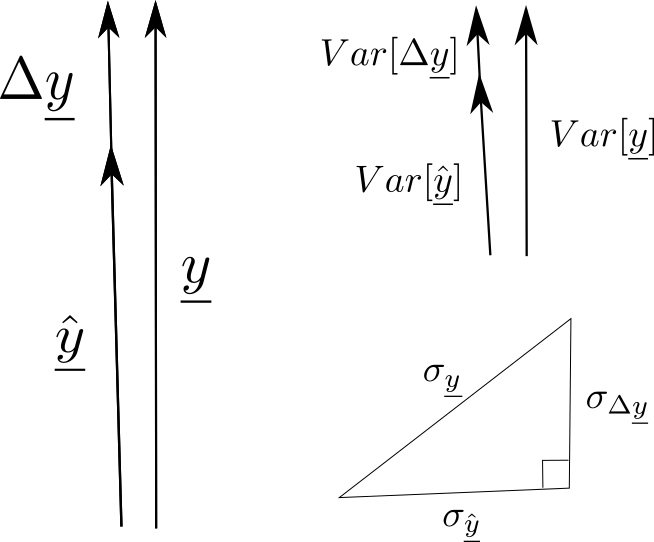
\includegraphics[width=2.3in]
{conventions/ms-error.png}
\caption{$\rvy=\hat{y}+\Delta y$
and the variances (not standard deviations)
of these quantities add. }
\label{fig-ms-error}
\end{figure}

\section{Cramer-Rao Bound}

This discussion of the Cramer-Rao (CR) bound
is based on Ref.\cite{wiki-cramer-rao}.

Suppose $\rvx$ is a random variable with values $x\in S_\rvx$
and $\theta\in\RR$ is a parameter.
For any function
$f_{\rvx,\theta}: S_\rvx\times \RR\rarrow \RR$,
define

\beq
\av{f_{\rvx,\theta}} =\sum_x P(x|\theta)f_{x,\theta}
\eeq

\beq
\Delta f_{\rvx,\theta}=f_{\rvx,\theta}-\av{f_{\rvx,\theta}}
\eeq

\beq
\av{f_{\rvx,\theta},f_{\rvx,\theta}}=
\av{\Delta f_{\rvx,\theta}\;\Delta f_{\rvx,\theta}}
\eeq

Define the {\bf log likelihood function} by
\beq
L_\theta = \ln P(x|\theta)
\eeq

Define the {\bf Fisher information} by
\beq
I_\theta=\av{\partial_\theta L_\theta,\partial_\theta L_\theta}
\eeq

Note that $L_\theta\leq 0$.
Let $\theta^*$ be the
value of $\theta$ that maximizes $L_\theta$.


Note that $I_\theta\geq 0$ and
$I_\theta=0$ when $\theta=\theta^*$
because $\partial_\theta L_\theta|_{\theta=\theta^*}=0$.
This suggests that $I_\theta$
measures the distance
between $\theta$ and $\theta^*$.



Note that
\beqa
\av{\partial_\theta L_\theta}&=&
\sum_x P(x|\theta)\frac{1}{P(x|\theta)}
\partial_\theta P(x|\theta)
\\
&=&
\partial_\theta \sum_x P(x|\theta)
\\
&=&
0
\eeqa
Therefore

\beqa
I_\theta &=&\av{[\partial_\theta L_\theta]^2}
-
\av{\partial_\theta L_\theta}^2
\\
&=&
\av{[\partial_\theta L_\theta]^2}
\eeqa

\begin{claim}
\beq
I_\theta = -\av{\partial_\theta^2 L_\theta}
\eeq
\end{claim}
\proof

\beqa
I_\theta &=& \av{[\partial_\theta L_\theta]^2}
\\
&=&
\sum_x P(x|\theta)
\frac{1}{P(x|\theta)}
\partial_\theta P(x|\theta)
\partial_\theta \ln P(x|\theta)
\\
&=&
-\sum_x P(x|\theta)\partial_\theta^2 \ln P(x|\theta)
+ \partial_\theta\sum_x
P(x|\theta)\partial_\theta \ln P(x|\theta)
\\
&=&
-\av{\partial_\theta^2 L_\theta}
+ \partial_\theta^2\sum_x P(x|\theta)
\\
&=&
-\av{\partial_\theta^2 L_\theta}
\eeqa
\qed

\begin{claim}
If $x=[x_i]_{i=1,2, \ldots \nu}\in \RR^\nu$ are i.i.d., then


\beq
I_\theta = \nu \av{[\partial_\theta L_{\theta, i}]^2}
\eeq
where

\beq
L_{\theta, i} = \ln P(x_i|\theta)
\eeq
\end{claim}
\proof

\beqa
L_\theta
&=& \ln \prod_i P(x_i|\theta)
\\
&=&
\sum_i L_{\theta, i}
\eeqa

\beqa
I_\theta &=&
\sum_i \sum_j \av{
\partial_\theta L_{\theta,i}
\partial_\theta L_{\theta,j}
}
\\
&=&
\sum_i  \av{
[\partial_\theta L_{\theta,i}]^2}
\\
&=&
\nu \av{
[\partial_\theta L_{\theta,i}]^2
}
\eeqa
\qed




A function  $t_\rvx:S_\rvx\rarrow \RR$
is called a {\bf test statistic} of random variable $\rvx$.

\begin{claim}(Cramer-Rao bound for single parameter $\theta\in\RR$)

\beq
\av{t_\rvx,t_\rvx}I_\theta \geq
 \left[\partial_\theta\av{t_\rvx}\right]^2
 \label{eq-crao-tx}
 \eeq
\end{claim}
\proof

Cauchy-Schwartz inequality

For two vectors $\veca,\vecb\in\RR^n$:
\beq
\veca\cdot\vecb =|\veca||\vecb|\cos \phi \leq |\veca||\vecb|
\eeq

For two real valued random variables $\rva, \rvb$:
\beq
\av{\rva, \rva} \av{\rvb,\rvb}\geq |\av{\rva,\rvb}|^2
\eeq
Replace

\beq
\rva\rarrow t_\rvx,
\quad\rvb\rarrow \partial_\theta L_\theta
\eeq
Then

\beqa
\av{t_\rvx, \partial_\theta L_\theta}
&=&
\av{t_\rvx \partial_\theta L_\theta}
-
\av{t_\rvx} \underbrace{\av{\partial_\theta L_\theta}}_{=0}
\\
&=&
\sum_x P(x|\theta)
t_\rvx \frac{1}{P(x|\theta)}\partial_\theta P(x|\theta)
\\
&=&
\partial_\theta\sum_x  t_\rvx P(x|\theta)
\\
&=&
\partial_\theta\av{ t_\rvx}
\eeqa
\qed

See Fig.\ref{fig-cramer-rao}
for a pictorial representation
of Eq.(\ref{eq-crao-tx}).

\begin{figure}[h!]
\centering
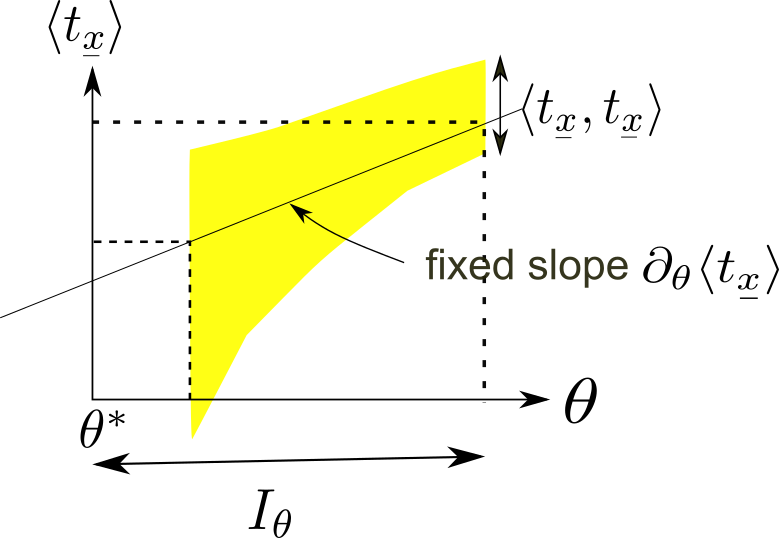
\includegraphics[width=2.7in]
{conventions/cramer-rao.png}
\caption{
In this drawing,
$\theta^*$ is the
value of $\theta$ that maximizes $L_\theta$.
According
to the CR bound,
the product of the
variance $\av{t_\rvx, t_\rvx}$ and
the distance $I_\theta$
must be greater or equal to $[\partial_\theta\av{t_\rvx}]^2$.
At fixed $[\partial_\theta\av{t_\rvx}]^2$,
if the variance increases, the distance decreases,
and vice versa.
}
\label{fig-cramer-rao}
\end{figure}


Now suppose the test statistic $t_\rvx$
equals an {\bf estimator} $\hat{\theta}$
of $\theta$ with bias $b_\rvx:S_\rvx \rarrow \RR$.

\beq
t_\rvx = \hat{\theta}(\rvx) = \theta + b_\rvx
\eeq
$\hat{\theta}$ is said to be a {\bf biased estimator}
if $b_\rvx\neq 0$ and an {\bf unbiased estimator} if $b_\rvx=0$.

\begin{claim}

\beq
\av{\hat{\theta}} = \theta + \av{b_\rvx}
\eeq

\beq
\av{\hat{\theta}, \hat{\theta}} \geq
\frac{[1 + \partial_\theta\av{b_\rvx}]^2}
{I_\theta}
\label{eq-crao-theta}
\eeq

\beq
\av{[\hat{\theta}-\theta]^2} \geq
\frac{[1 + \partial_\theta\av{b_\rvx}]^2}
{I_\theta}
+
\av{b_\rvx}^2
\eeq

\end{claim}
\proof
\beqa
\partial_\theta\av{t_\rvx}
&=&
\partial_\theta\av{\theta + b_\rvx}
\\
&=&
\partial_\theta\left[\theta +\av{b_\rvx}\right]
\\
&=&
1 + \partial_\theta\av{b_\rvx}
\eeqa
Eq.(\ref{eq-crao-theta})
follows from Eq.(\ref{eq-crao-tx})
once we replace $t_\rvx$ by $\hat{\theta}$.

Let
\beq
\Delta \hat{\theta} =
\hat{\theta} -\av{\hat{\theta}}
=
\underbrace{(\hat{\theta} -\theta)}_\xi  - \av{b_\rvx}
\eeq
Then

\beq
0=\av{\Delta \hat{\theta}} = \av{\xi} - \av{b_\rvx}
\eeq

\beqa
\frac{[1 + \partial_\theta\av{b_\rvx}]^2}
{I_\theta} &\leq&
\av{[\Delta \hat{\theta}]^2}
\\
&=&
\av{\xi^2 -2\xi\av{b_\rvx} + \av{b_\rvx}^2}
\\
&=&
\av{\xi^2} -\av{b_\rvx}^2
\eeqa

\qed

Multi-dimensional case:
parameter
 $\theta=[\theta_1, \theta_2, \ldots, \theta_n]^T\in \RR^n$
 and test statistic
 $t_\rvx=[t_{\rvx,1}, t_{\rvx,2}, \ldots, t_{\rvx,n}]^T\in \RR^n$
are column vectors.

Define {\bf Fisher information matrix} by

\beq
[I_\theta]_{i,j}=
\av{\partial_{\theta_i} L_\theta, \partial_{\theta_j}L_\theta}
=
\av{\partial_{\theta_i} L_\theta\;\partial_{\theta_j}L_\theta}
\eeq

CR bound for multi-dimensional parameter $\theta\in\RR^n$:
\beq
\text{matrix}\left[\av{t_{\rvx,i}, t_{\rvx,j}}\right]\geq
\text{matrix}\left[
\partial_{\theta_i} \av{t_{\rvx,a}}
[I_\theta]^{-1}_{a,b}
\partial_{\theta_j} \av{t_{\rvx,b}}
\right]
\eeq
where we are using the Einstein summation
convention (repeated indices are summed over).
For two matrices $A,B\in\RR^n$, $A\geq B$ means $A-B$ has
non-negative eigenvalues.


\section{Bayes Rule,
Bayesian Updating And Conjugate Priors}

Bayes Rule says:

\beq
P(\theta|x)P(x)
=
P(x|\theta)P(\theta)
\eeq
Expressed diagramatically\footnote{Two bnets are equated if their full probability
distributions (i.e.,
their full instantiations) are equal numerically.},
we have for  $\rvx\in\RR$:
\beq
\xymatrix{
\rvtheta&\rvx\ar[l]
}
\quad =\quad
\xymatrix{
 \rvtheta\ar[r]&\rvx
}
\eeq
and for $\rvx=(\rvx_1, \rvx_2)\in \RR^2$:
\beq
\begin{array}{c}
\xymatrix@R=.3pc{
&\rvx_1\ar[ld]\ar[dd]
\\
\rvtheta
\\
&\rvx_2\ar[lu]
}
\xymatrix@R=.3pc{\\\quad =\quad}
\xymatrix@R=.3pc{
&\rvx_1\ar[dd]
\\
\rvtheta\ar[ru]\ar[rd]
\\
&\rvx_2
}
\end{array}
\eeq
Note how Bayes rule
allows us to reverse the
direction of the arrows
impinging on $\theta$.
We see from Bayes Rule
that even though
the directions of
the arrows in a
bnet can have causal
motivation, a bnet
with arrows reversed
from their causally
motivated directions
can still be very useful
as a calculation tool.

Another way of stating
Bayes Rule is




\beq
\underbrace{P(\theta|x)}_{\rm posterior}=
\caln(!\theta)
\underbrace{P(x|\theta)}_{\rm likelihood}
\underbrace{P(\theta)}_{\rm prior}
\;.
\eeq

If, for a given likelihood,
the prior and posterior
distributions belong to
the same family (for instance,
they are both
Beta distributions),
then we say that the prior is the
{\bf conjugate prior}
of that likelihood.

For example,
Beta $\sim$ Bernoulli*Beta.
Hence, the
Beta distribution\footnote{See
Ref.\cite{wiki-beta-dist} for a discussion
of the Beta distribution.}
is the conjugate prior of the
Bernoulli distribution\footnote{See
Ref.\cite{wiki-bern-dist} for a discussion
of the Bernoulli distribution}.
More explicitly,
if

\beq
p_1\sim {\rm Beta}(p_1;\alp, \beta)
\eeq
and

\beq
x|p_1\sim {\rm Bernoulli}(x;p_1)
\;,
\eeq
where $p_1=P(x=1)$,
then

\beq
p_1|x\sim {\rm Beta}(p_1;\alp', \beta')
\eeq
where

\beq
\alp'= \alp + x
\eeq

\beq
\beta'= \beta + (1-x)
\eeq


Ref.\cite{wiki-conj-prior}
has a table of
conjugate priors.

Conjugate priors facilitate
Bayesian updating
of the prior to
posterior in a
feedback loop(see Fig.\ref{fig-conj-prior}).

\begin{figure}[h!]
$$\xymatrix{
&x_t\ar[d]
\\
&\stackrel{Bernoulli}{P(x_t|\theta)}\ar@/_2pc/[ld]
\\
\stackrel{Beta}{P(\theta|x_{\leq t})}\ar@/_2pc/[rd]
&&\stackrel{Beta}{P(\theta|x_{\leq t-1})}\ar@/_2pc/[ul]
\\
&t\rarrow t+1 \text{ for } t=0, 1, 2,\ldots
\ar@/_2pc/[ur]
}$$
\caption{Bayesian updating facilitated
by conjugate prior. In this figure,
$x_{\leq t}=(x_0, x_1, \ldots, x_{t-1}, x_t)$.}
\label{fig-conj-prior}
\end{figure}


\section{Linear regression, Ordinary Least Squares (OLS)}
\label{sec0-conv-lr}
Wikipedia articles
\begin{enumerate}
\item
Linear Regression (LR)
\begin{itemize}
\item
linear regression, Ref.\cite{wiki-lr}
\item
 simple linear regression, Ref.\cite{wiki-slr}
\item
errors in variable, Ref.\cite{wiki-errors-in-iv}

\end{itemize}
\item
Least squares (LS)
\begin{itemize}
\item
least squares, Ref.\cite{wiki-lsquares}
\item
ordinary least squares (OLS), Ref.\cite{wiki-ols}
\end{itemize}
\end{enumerate}


Some nomenclature: In LR, the
data consists of
{\bf independent x-variables} $x^\s_1,
 x^\s_2, \ldots x^\s_n$
and a {\bf dependent y-variable} $y^\s$.
We find a linear fit $\haty^\s =
\beta_0 + \sum_{i=1}^n \beta_i x^\s_i$
to the data.
$\haty^\s$ is called the {\bf estimate}
of $y^\s$.
 The coefficients $\beta_0, \beta_i$
are called {\bf regression coefficients}.
$y^\s-\haty^\s=\eps^\s$
are called  the {\bf residuals}.
$\cale =\sum_\s (\eps^\s)^2$
is called the {\bf error or cost}. We choose the
regression coefficients
so as to minimize the error.

Below, we consider two types of LR:

\begin{enumerate}
\item
LR
in which the independent x-variables are non-random.
\item
LR
in which the independent x-variables are random
and i.i.d.
\end{enumerate}

The  term OLS
is often used to refer to LR
of type 1.



For LR of type 2,
there is randomness in $y$
coming from the randomness in $x$
and in the residuals.
For LR of type 1,
there  is randomness in $y$
too, but
it comes
from the residuals
only.

Once one assumes that certain
variables are random, a
``model" (i.e., a bnet,
with probabilities expressed as TPMs)
 must be
specified.


\subsection{LR, assuming
$x_\s$ are non-random}

Let

$\s\in\{0, 1, 2, \ldots, nsam-1\}$ : sample index

$i_0\in\{0, 1, 2, \ldots, n\}$ :
index that can assume values 0 to $n$

$i\in\{1, 2, \ldots, n\}$ :
index that can assume values 1 to $n$.
$i$ is never equal to 0.


$y_\s\in \RR$: dependent y-variables

$x_{\s i}\in \RR$: independent x-variables

$\eps_\s\in \RR$: residuals

$\beta_0, \beta_i\in \RR$:
regression coefficients


\beq
y_\s= \beta_0 +
\sum_{i=1}^{n} x_{\s i}\beta_{i} + \eps_\s
\label{eq-LR-start}
\eeq

If we define
\beq
x_{\s 0}=1
\;
\eeq
for all $\s$, then

\beq
y_\s=
\sum_{i_0=0}^{n} x_{\s i_0}\beta_{i_0} + \eps_\s
\;.
\eeq
If $y$ and $\eps$ are $nsam$ dimensional
 column vectors and $\beta$
is an $n+1$ dimensional column vector,
and $X$ is an $nsam\times (n+1)$ matrix,
then we can write the previous equation in matrix
form as:


\beq
y=X\beta+\eps
\;.
\eeq

\subsubsection{Derivation of LR
 From Minimization of Error}

Let $W=[W_{\s, \s'}]$
be a symmetric matrix with non-negative
diagonal elements $W_{\s,\s}\geq 0$ for all $\s$.
$W$ is called the {\bf weight matrix}.
The following claim
describes the method of
{\bf Weighted LR}
when $W\neq 1$
and of simple LR  when $W=1$.
\begin{claim}
Assume the
Einstein summation convention; i.e.,
implicit sum over
repeated indices.
The
 error function $\cale$ given by

\beq
\cale=
\underbrace{(y_{\s}-X_{\s, j_0}\beta_{j_0})}
_{\text{residual $\eps_\s$}}
W_{\s, \s'}
\underbrace{(y_{\s'}-X_{\s', k_0}
\beta_{k_0})}_{\eps_{\s'}}
\;,
\eeq
is minimized
over $\beta_{k_0}$ for all $k_0
\in\{0,1,\ldots,n\}$,
if $\beta_{k_0}$ is given by:

\beq
\hat{\beta}= (X^T W X)^{-1} X^T W y
\;.
\label{eq-betahat-non-ran-w}
\eeq
When $W=1$,

\beq
\hat{\beta}= (X^T X)^{-1} X^T y
\;.
\label{eq-betahat-non-ran}
\eeq

\end{claim}
\proof

At the minimum of $\cale$,
the variation $\delta\cale$
 must vanish:
\beq
0=\delta \cale=
-2 X_{\s j_0}(\delta \beta_{j_0})
W_{\s, \s'}(y_{\s'}
-X_{\s' k_0}
\beta_{k_0})
\;.
\eeq
Thus,

\beq
X^T W y - X^T W X\beta=0
\eeq
which
implies Eq.(\ref{eq-betahat-non-ran-w}).
\qed

\subsubsection{Geometry of LR
with non-random $x_\s$.}

Recall that

\beq
y=X\beta+\eps
\;.
\eeq


Define the {\bf projection matrices}

\beq
\A=X(X^TX)^{-1}X^T
\;,\;\;\V=1-\A
\eeq
A square matrix $M$
is symmetric if $M^T=M$
and is idempotent if $M^2=M$.
$\A$ is symmetric
and idempotent
and so is $\V$.
Note that $\A$ and $\V$
also satisfy:

\beq
\V\A=\A\V=0
\eeq
and

\beq
\A X=X\;,\;\; \V X=0
\;.
\eeq

One has

\beq
\beta=
(X^TX)^{-1}X^T(y-\eps)
\;.
\eeq


Define

\begin{subequations}
\beq \boxed{
\hat{\beta}=
\underbrace{(X^TX)^{-1}X^T}_B \;y
\;,
}
\label{eq-beta-nonrandom-lin-reg}
\eeq



\beq
\hat{y}=
X\hat{\beta}= \A y
\;,
\eeq
and

\beq
\hat{\eps}=
y-X\hat{\beta}=
y-\hat{y}=(1-\A)y=\V y
\;.
\eeq
\end{subequations}
$\A$ is sometimes  called the {\bf hat matrix},
because it gives $y$ a hat.

Given any function $f=f(y,X,\eps)$
and a scalar factor $\xi\in \RR$,
suppose
$f(\xi y, \xi X, \xi\eps)=\xi^\calo f(y,X,\eps)$.
Then we will say that $f(\cdot)$
is of {\bf order $\calo$ under scaling}.
Note that $\{\hat{y},
 \hat{\eps}\}$
are all of order 1 under scaling,
$\{\beta, \hat{\beta}, \A, \V\}$
are all of order 0 under scaling,
and $B$ is of order $-1$ under scaling.
Thus, each cfit (i.e., symbol
with a hat)
scales the same way as its estimand (i.e., same
symbol
without a hat). Furthermore,
$\beta$, its cfit $\hat{\beta}$, and
the projection matrices $\A, \V$
are invariant ($\calo=0$) under scaling.



Note that $y$
can be expressed as
a sum of 2 orthogonal estimates:



\beq
y= \underbrace{\hat{y}}_{\A y} +
\underbrace{\hat{\eps}}_{\V y}
\;.
\eeq
Fig.\ref{fig-lin-reg-vecs}
shows triangles representing
$y=X\beta+\eps$ and $y=\hat{y}+\hat{\eps}$.


\begin{figure}[h!]
\centering
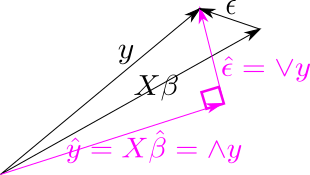
\includegraphics[width=2in]
{conventions/lin-reg-vecs.png}
\caption{Triangles
representing
$y=X\beta+\eps$ and $y=\hat{y}+\hat{\eps}$.}
\label{fig-lin-reg-vecs}
\end{figure}

\subsubsection{LR Goodness of Fit, $R^2$}


Assume the components of $\eps$
are random with zero mean:

\beq
E[\rveps]=\av{\rveps}=0
\eeq



Assume $X$ and $\beta$ are not random.
This makes $\rvy=X\beta +\rveps$ and $\ul{\hat{\beta}}=
(X^TX)^{-1}X^T\rvy
$
random.
One finds that

\begin{subequations}
\beq
\av{\rvy}=X\beta
\eeq


\beq
\av{\hat{\rvy}}=\A
\underbrace{\av{\rvy}}_{X\beta}
=\av{\rvy}
\eeq

\beq
\av{\hat{\rveps}}=\V
\underbrace{\av{\rvy}}_{X\beta}
=0
\eeq

\beq
\av{\ul{\hat{\beta}}}=\beta
\eeq


So far, we have
assumed a zero mean value for $\eps$.
Next, assume
{\bf  ``homoscedasticity" (homo-spread)}\footnote{I
 find the word ``homoscedasticity"
unnecessarily long, cryptic
and easy to misspell so
I like to replace
it by ``homo-spread".
The opposite
of ``homoscedasticity"
is ``heteroscedasticity",
which I like to replace with ``hetero-spread".}, which
means that

\beq
\av{\rveps, \rveps^T}=\xi^2 I_{nsam}
\eeq
\end{subequations}
where
$\xi\geq 0$,  and
$I_{nsam}$ is the
$nsam\times nsam$ identity matrix.
It follows that

\begin{subequations}
\label{eq-lin-re-variances}
\beq
\av{\rvy, \rvy^T}=
\av{\rveps, \rveps^T}=
\xi^2 I_{nsam}
\;,
\eeq

\beq
\av{\hat{\rveps},
\hat{\rveps}^T}=
\V\av{\rvy, \rvy^T}\V^T=\xi^2\V
\label{eq-homo}
\;,
\eeq

\beq
\av{\hat{\rvy},
\hat{\rvy}^T}=
\A\av{\rvy, \rvy^T}\A^T=\xi^2\A
\eeq
and

\beq
\av{\hat{\ul{\beta}},
\hat{\ul{\beta}}^T}=
B\av{\rvy, \rvy^T}B^T=\xi^2 (X^TX)^{-1}
\;.
\eeq
\end{subequations}

For any random column vector $\rva$,
let

\beq
\norm{\rva}^2= \rva^T\rva=\tr(\rva\rva^T)
\eeq
and

\beq
\av{\norm{\rva-\av{\rva}}^2}=
\av{\rva^T\rva}-\av{\rva^T}\av{\rva}
=
\tr\av{\rva, \rva^T}
\;.
\eeq

Define the following sums of squares (SS):

\begin{subequations}
\label{eq-lin-reg-ss}
\beq
SS_{\rvy}=\av{\norm{\rvy-\av{\rvy}}^2}
=\av{\rvy^T\rvy}-\av{\rvy^T}\av{\rvy}
=\tr\av{\rvy,\rvy^T}
\eeq

\beq
SS_{\hat{\rvy}}=\av{\norm{\hat{\rvy}-\av{\hat{\rvy}}}^2}
=\av{\hat{\rvy}^T\hat{\rvy}}-\av{\hat{\rvy}^T}\av{\hat{\rvy}}
=\tr\av{\hat{\rvy},\hat{\rvy}^T}
\eeq

\beq
SS_{res}=\av{\norm{\rvy-\hat{\rvy}}^2}
=
\av{\norm{\ul{\hat{\eps}}}^2}
=\tr\av{\ul{\hat{\eps}},\ul{\hat{\eps}}^T}
\eeq
\end{subequations}

\begin{claim}
The following is true
without homo-spread:


\beq
\underbrace{\tr\av{\rvy,\rvy^T} }_{SS_\rvy}
=
\underbrace{\tr\av{\hat{\rvy}, \hat{\rvy}^T}}_{SS_{\hat{\rvy}}}
+
\underbrace{\tr\av{\hat{\rveps}, \hat{\rveps}^T}}_{SS_{res}}
\eeq
This is like the Pythagorean Theorem
for the magenta right triangle
in Fig.\ref{fig-lin-reg-vecs}.
\end{claim}
\proof

From Eqs.\ref{eq-lin-re-variances}
and \ref{eq-lin-reg-ss},
we see that

\beq
SS_\rvy=\tr\av{\rvy,\rvy^T}
\eeq

\beq
SS_{\hat{\rvy}}=\tr\av{\hat{\rvy},\hat{\rvy}^T}
=\tr\av{\A\rvy, \rvy^T}
\eeq

\beq
SS_{res}=\tr\av{\hat{\rveps}, \hat{\rveps}^T}
=\tr\av{\V\rvy, \rvy^T}
\eeq
Now use $\A + \V=1$.
\qed


The goodness of fit
for this model
is often measured using  the
{\bf coefficient of determination}
$R^2$. $R^2$  is defined by


\beq
R^2= 1 -\frac{SS_{res}}{SS_\rvy}=
\frac{SS_{\hat{y}}}{SS_\rvy}
=
\frac{\tr \av{\hat{\rvy},\hat{\rvy}^T}}
{ \tr \av{\rvy,\rvy^T}}
\eeq
If homo-spread holds, then
$R^2$ reduces to


\beq
R^2 =\frac{\tr\; \A}{nsam}
\;.
\eeq


\subsection{LR, assuming
$x_\s$ are random}
Let

$i_0\in\{0, 1, 2, \ldots, n\}$ :
index that can assume values 0 to $n$

$i\in\{1, 2, \ldots, n\}$ :
index that can assume values 1 to $n$.
$i$ is never equal to 0.


$\rvy\in\RR$:  true value
of dependent y-variable

$\hat{\rvy}\in\RR$: cfit
of dependent y-variable

$\ul{\eps}\in\RR$: residual



$\rvx_{i}\in \RR$: independent x-variables
for $i\in\{1,\ldots,n\}$

$\beta_0, \beta_i\in\RR$:
regression coefficients

\beqa
\hat{\rvy}
&=&
\beta_0 +\sum_{j=1}^{n}
\beta_{j} \rvx_j
\\
&=&
\sum_{j_0=0}^{n}\beta_{j_0} \rvx_{j_0}
\;\;(\text{Assume $\rvx_0=1$.})
\eeqa

\beq
\rvy = \hat{\rvy}+\ul{\eps}
\eeq

\subsubsection{Transforming
expressions
from
non-random to
random $x_\s$ }

Define the following
population averages:


\beq
E_\s[x^\s]=
\frac{1}{nsam}
\sum_\s x^\s
\;,
\eeq

\beq
E_\s[x^\s y^\s]=
\frac{1}{nsam}
\sum_\s x^\s y^\s
\;,
\eeq

\beq
\av{x^\s,y^\s}_\s=
E_\s[x^\s y^\s]-E_\s[x^\s]E_\s[y^\s]
\;.
\eeq


\begin{claim}\label{cl-sigma-to-ran}
If the $x_\s$ are i.i.d. random
variables,

\beq
E_\s[x^\s] =\av{\rvx}
\;
\label{eq-exp-x}
\eeq
\beq
E_\s[x^\s y^\s]
=
\av{\rvx\rvy}
\label{eq-exp-xy}
\eeq

\beq
\av{x^\s,y^\s}_\s
=
\av{\rvx, \rvy}
\label{eq-exp-x--y}
\eeq
\end{claim}
\proof
\beqa
\frac{1}{nsam}
\sum_\s x^\s
&=&
\frac{1}{nsam}
\sum_{x\in S_\rvx}
x
\underbrace{
\sum_\s \indi(x^\s=x)}_
{N(x^\s=x)}
\\
&=&
\sum_{x}x\;P(x)
\\
&=&
\av{\rvx }
\eeqa

\beqa
\frac{1}{nsam}
\sum_\s x^\s y^\s
&=&
\frac{1}{nsam}
\sum_{x\in S_\rvx}
\sum_{y\in S_\rvy}
xy
\underbrace{
\sum_\s \indi(x^\s=x, y^\s=y)}_
{N(x^\s=x, y^\s=y)}
\\
&=&
\sum_{x,y}xy\;P(x,y)
\\
&=&
\av{\rvx \rvy}
\eeqa
Eq.(\ref{eq-exp-x--y})
follows from
Eq.(\ref{eq-exp-x}) and Eq.(\ref{eq-exp-xy}).
\qed

Recall that

\beq
Y_\s = \beta_0 +  \sum_{j=1}^n X_{\s,j}\beta_j + \eps_\s
\;.
\eeq

Assume
\beq
E_\s[X_{\s,k} \eps_\s]=E_\s[X_{\s,k}]
\underbrace{E_\s[ \eps_\s]}_{=0}=0
\;.
\eeq
Then we have

\beq
E_\s[X_{\s,k} Y_\s]=
E_\s[X_{\s,k}]\beta_0 + \sum_{j=1}^n
E_\s [X_{\s,k} X_{\s,j}] \beta_j +
\underbrace{E_\s[X_{\s,k} \eps_\s]}_{=0}
\label{eq-EXY}
\eeq
and

\beq
E_{\s'}[X_{\s',k}]E_\s[ Y_\s]=
E_{\s'}[X_{\s',k}]\beta_0 + \sum_{j=1}^n
E_{\s'} [X_{\s',k}] E_\s[ X_{\s,j}] \beta_j +
\underbrace{E_{\s'}[X_{\s',k}]  E_\s[ \eps_\s]}_{=0}
\label{eq-EX-EY}
\;.
\eeq
Subtracting
Eq.(\ref{eq-EX-EY}) from Eq.(\ref{eq-EXY}), we get

\beq
\av{X_{\s,k} ,Y_\s}_\s=
\sum_{j=1}^n
\av{X_{\s,k}, X_{\s,j}}_\s \beta_j
\label{eq-avX-comma-Y}
\;.
\eeq
Define the $n$ dimensional
covariance matrix $C$
by

\beq
C_{k,j}=\av{X_{\s,k}, X_{\s,j}}_\s
\:.
\eeq
Then Eq.(\ref{eq-avX-comma-Y}) implies

\beq
\beta_j =\sum_{k=1}^n
C^{-1}_{j,k} \av{X_{\s,k} ,Y_\s}_\s
\label{eq-beta_j-c-inv}
\eeq
for all $j=1,2,\ldots, n$.

If we assume that the $x_\s$ are i.i.d.,
then, by  virtue of Claim \ref{cl-sigma-to-ran},
the matrix $C$ tends to


\beq
C_{k,j}
\rarrow \av{\rvx_k, \rvx_j}
\eeq
and Eq.(\ref{eq-beta_j-c-inv})
implies

\beq
\beta_j = \sum_{k=1}^n C^{-1}_{j,k}\av{\rvx_k, \rvy}
\label{eq-beta-random-from-nonrandom}
\;.
\eeq

\subsubsection{Geometry of LR with random $x_\s$}
Recall that

\beq
\rvy =
\underbrace{\beta_0 +\sum_{j=1}^{n}
\beta_{j} \rvx_j}_{\hat{\rvy}}
+\ul{\eps}
\;.
\eeq


Assume

\beq
\av{\rveps}=0
\eeq
and
\beq
\av{\rvx_j, \ul{\eps}}=0
\eeq
for all $j$.

For $k=1, \ldots, n$,
\beq
\av{\rvx_k, \rvy}
=
\sum_{j=1}^{n}\beta_j\av{\rvx_k, \rvx_j}
\;.
\label{eq-beta-0-wrong}
\eeq

Let $\rvx^n$ and $\beta^n$ be
$n$-dimensional column vectors.
Then Eq.(\ref{eq-beta-0-wrong})
can be represented
 in matrix notation by
\beq
\av{\rvx^n, \rvy}=
\av{\rvx^n, (\rvx^n)^T}\beta^n
\;.
\eeq
Hence,

\beq
\boxed{
\beta^n=
\av{\rvx^n, (\rvx^n)^T}^{-1}
\av{ \rvx^n, \rvy}
\;.}
\label{eq-beta-random-lin-reg}
\eeq
For $\beta_0$, use

\beq
\beta_0=
\av{\rvy}-\av{\rvx^n}^T \beta^n
\eeq

Notice that
Eq.(\ref{eq-beta-random-lin-reg})
for the regression coefficients
is the same
as Eq.(\ref{eq-beta-random-from-nonrandom}).
So we have rederived the same formula
via a different method.


Next, we will
write
 Eq.(\ref{eq-beta-random-lin-reg})
for the special cases
$n=1$ and $n=2$,
where $n$ is the
number of independent x-variables $\rvx_j$

\begin{enumerate}
\item $n=1$ ($\rvy$ fitted by a line)

\beq
\rvy = \beta_0 + \beta_1\rvx + \rveps
\eeq

Eq.(\ref{eq-beta-random-lin-reg}) becomes
\beq
\beta_1=
\frac{\av{\rvy,\rvx}}{\av{\rvx,\rvx}}
\eeq


\item $n=2$ ($\rvy$ fitted by a plane)


\beq
\rvy = \beta_0 + \beta_1 \rvx_1 + \beta_2 \rvx_2 +\rveps
\eeq
Define


\beq
C_{i,j}=\av{\rvx_i, \rvx_j}
\eeq
for all $i,j$.
Then Eq.(\ref{eq-beta-random-lin-reg})
becomes\footnote{
Recall that if
$
M=
\left[
\begin{array}{cc}
a&b
\\
c&d
\end{array}
\right]
$
then
$
M^{-1}
=
\frac{1}{\det M}
\left[
\begin{array}{cc}
d&-b
\\
-c&a
\end{array}
\right]
$
}


\beqa
\left[
\begin{array}{c}
\beta_1
\\
\beta_2
\end{array}
\right]
&=&
C^{-1}
\left[
\begin{array}{c}
\av{\rvy, \rvx_1}
\\
\av{\rvy, \rvx_2}
\end{array}
\right]
\\
&=&
\frac{1}{\det C}
\left[
\begin{array}{cc}
C_{22}&-C_{12}
\\
-C_{21}&C_{11}
\end{array}
\right]
\left[
\begin{array}{c}
\av{\rvy, \rvx_1}
\\
\av{\rvy, \rvx_2}
\end{array}
\right]
\eeqa


Hence,
\beq
\beta_1
=\pder{\rvy}{\rvx_1}=
\frac{
C_{22}\av{\rvy, \rvx_1}
-C_{12}\av{\rvy, \rvx_2}
}
{
C_{11}C_{22}-C_{12}^2
}
\label{eq-beta-lr-plane}
\eeq
Eq.(\ref{eq-beta-lr-plane})
 agrees with
the
value of $\beta_{YX, Z}$ in
Ref.\cite{pearl-lin-reg}
by Pearl,
if  we replace in Pearl's
formulae $X\rarrow \rvx_1$,
$Y\rarrow \rvy$, $Z\rarrow \rvx_2$.


\end{enumerate}

\subsubsection{Regression
 interpreted as differentiation
 of $y$}

Finding the derivative of $y$
with respect to (wrt) $X$
(a.k.a. ``{\bf Regressing $y$ on $X$}")
is finding
$\hat{\beta}=\frac{d}{dX}
\underbrace{y}_{X\beta}$.

Recall that

\beq
\rvy = \beta_0 + \sum_{k=1}^n \rvx_k \beta_k + \ul{\eps}
\;.
\eeq
Therefore,

\beqa
\av{\rvx_i, \rvy}
&=&
\sum_{k=1}^n \av{\rvx_i, \rvx_k}\beta_k
\\
&=&
 \av{\rvx_i, \rvx_i}\beta_i
+
\sum_{k=1}^n
\indi(k\neq i)
 \av{\rvx_i, \rvx_k}\beta_k
\;.
\eeqa
Hence,

\beq
\beta_i
=
\frac{\av{\rvx_i, \rvy}}
{\av{\rvx_i, \rvx_i}}
-\sum_{k=1}^n
\indi(k\neq i)
\frac{ \av{\rvx_i, \rvx_k}}
{\av{\rvx_i, \rvx_i}}
\beta_k
\;.
\label{eq-beta-i-non-deriv}
\eeq

Let's represent
the linear
operator
$\av{\rvx_i, \rvx_i}^{-1}\av{\rvx_i, \cdot}
$ as a derivative:

\beq
\frac{d\;\cdot}{d\rvx_i}=
\frac{\av{\rvx_i, \cdot}}
{\av{\rvx_i, \rvx_i}}
\;.
\eeq
Eq.(\ref{eq-beta-i-non-deriv})
can be expressed
in derivative notation as:

\beq
\beta_i
=
\frac{d \rvy}
{d\rvx_i}
-\sum_{k=1}^n\indi(k\neq i)
\frac{ d\rvx_k}
{d\rvx_i}
\beta_k
\label{eq-beta-i-deriv}
\eeq
Note that Eq.(\ref{eq-beta-i-deriv})
evokes the formula for differentials:

\beq
d\rvy=
\sum_{k=1}^n \beta_kd\rvx_k
\;.
\eeq

Note also that,
because of the
linearity of the derivative operator,
Eq.(\ref{eq-beta-i-deriv})
implies:

\beq
\beta_i=
\frac{d}
{d\rvx_i}
\left(\rvy
-
\underbrace{\sum_{k=1}^n
\indi(k\neq i)\rvx_k \beta_k
}_{\rvy-\rvx_i\beta_i}
\right)
\label{eq-beta-i-2-steps}
\;.
\eeq

Eq.(\ref{eq-beta-i-2-steps})
can be used to find
$\hat{\beta}_i$
in two steps:

STEP 1: Regress $\rvy-\rvx_i\beta_i$
on $(\rvx_k)_{k\in \{1,2,
\ldots, n\}- \{ i\}}$.
Get estimates
$(\hat{\beta}_k)_{k\in \{1,2,
\ldots, n\}- \{ i\}}$.

STEP 2: Regress $\rvy-\sum_{k\neq i} \rvx_k\hat{\beta}_k$ on $\rvx_i$.
Get estimate $\hat{\beta}_i$.

Of course, one can also
find $\hat{\beta}_i$
by regressing $\rvy$
on $(\rvx_k)_{k\in \{1,2,
\ldots, n\}}$, to get
estimates
$(\hat{\beta}_k)_{k\in \{1,2,
\ldots, n\}}$.

\section{Logistic Regression (LoR)}

Suppose
$x_\s\in \RR^n$,
$y_\s\in \RR$,
and $\Sigma$
is a population
of individuals $\s$.
In general,
a {\bf regression}
is when
we curve-fit a dataset
$\{(x_\s, y_\s):\s\in\Sigma\}$
with a function
$\haty=f(x)$.
In {\bf Linear
Regression (LR)},
which we
discussed earlier,
$f(x)$ is a hyperplane
in $x$.
On the other hand,
in {\bf Logistic Regression (LoR)},
$y_\s\in[0,1]$ and
$f(x)$ is the sigmoid of
a hyperplane in $x$.



More specifically, for LR
we have
Eq.(\ref{eq-LR-start})
which reads as follows:

\beq
y_\s=
\underbrace{
\beta_0 +
\sum_{i=1}^{n} x_{\s i}\beta_{i}
}_{\haty_\s}+ \eps_\s
\quad\text{(LR)}\;.
\eeq
For LoR, we have instead

\beq
p_\s=
\smoid\left(
\beta_0 +
\sum_{i=1}^{n} x_{\s i}\beta_{i} + \eps_\s
\right)
\quad\text{(LoR)}\;,
\eeq
or, equivalently,


\beq
\underbrace{\lodds(p_\s)}
_{\ln \frac{p_\s}{1-p_\s}}=
\underbrace{
\beta_0 +
\sum_{i=1}^{n} x_{\s i}\beta_{i}
}_{\haty_\s} + \eps_\s
\quad\text{(LoR)}\;,
\eeq
where we have used the fact that
$\lodds()$
is the inverse function of $\smoid()$.
Hence, an LoR
fit can be calculated by
collecting a dataset
$\{(x_\s, p_\s):\s\in\Sigma\}$,
transforming that
dataset to the dataset
$\{(x_\s,\lodds( p_\s)):\s\in\Sigma\}$,
and fitting the latter dataset
with a hyperplane.
Let $P(\rvY_\s=1)=p_\s\in [0,1]$.
LoR can be used
for binary
classification
if we define the
binary class
variable $c_\s\in \bool$ by

\beq
c_\s =\indi(P(\rvY_\s=1)>\alp)
\eeq
for some $0<\alp<1$.



\section{Entropy,
 Kullback-Liebler divergence, Cross-Entropy}

For probability distributions $p(x), q(x)$ of $x\in S_\rvx$
\begin{itemize}
\item
Entropy:
\beq
H(p)=-\sum_x p(x)\ln p(x)\geq 0
\eeq

\item
Kullback-Liebler divergence:

\beq
D_{KL}(p\parallel q)=\sum_{x} p(x)\ln \frac{p(x)}{q(x)}\geq 0
\eeq
\item
Cross entropy:
\beqa
CE(p\parallel q) &=& -\sum_x p(x)\ln q(x)\\
&=& H(p) + D_{KL}(p\parallel q)
\eeqa
\end{itemize}

\section{Definition of various
entropies used in Shannon Information Theory}

\begin{itemize}
\item
{\bf (plain) Entropy of $\rvx$}

\beq
H(\rvx) =
-\sum_{x} P(x)\ln P(x)
\eeq
This quantity measures the
spread of $P_\rvx$.
$H(\rvx)\geq 0$
and it vanishes iff $P(x)=\delta(x,x_0)$ (deterministic case)


\item
{\bf Conditional Entropy of $\rvy$ given $\rvx$}

\beqa
H(\rvy|\rvx) &=&
-\sum_{x,y}P(x,y)\ln {P(y|x)}
\\
&=&
H(\rvy,\rvx)-H(\rvx)
\eeqa
This quantity measures  the conditional
 spread
of $\rvy$ given $\rvx$. $H(\rvy|\rvx)\geq 0$.


\item {\bf Mutual Information (MI)
of $\rvx$ and $\rvy$}.

\beqa
H(\rvy:\rvx) &=&
\sum_{x,y} P(x,y) \ln \frac{P(x,y)}{P(x)P(y)}
\\
&=&
H(\rvx) + H(\rvy) - H(\rvy,\rvx)
\eeqa
This quantity measures the correlation
between $\rvx$ and $\rvy$.
$H(\rvy:\rvx)\geq 0$
and it vanishes iff
$P(x,y)=P(x)P(y)$.

\item {\bf Conditional Mutual Information
(CMI)\footnote{CMI
can be read as ``see me".}
of $\rvx$ and $\rvy$
given $\ul{\lam}$}


\beqa
H(\rvy:\rvx|\ul{\lam})
&=&
\sum_{x,y, \lam}P(x,y, \lam) \ln
\frac{P(x,y|\lam)}{P(x|\lam)P(y|\lam)}
\\
&=&
H(\rvx|\ul{\lam}) + H(\rvy|\ul{\lam})
- H(\rvy,\rvx|\ul{\lam})
\eeqa

This
quantity measures the conditional correlation
of $\rvx$ and $\rvy$ given $\ul{\lam}$.
$H(\rvy:\rvx|\ul{\lam})\geq 0$
and it vanishes iff
$P(x,y|\lam)=P(x|\lam)P(y|\lam)$.

An interesting special case
occurs when
$P(\lam)=\delta(\lam, \lam_0)$ (the
frequentist  case of no $\lam$ prior.)
In that case CMI
reduces to

\beq
H(\rvy:\rvx|\lam_0)
=
\sum_{x,y}P(x,y|\lam_0) \ln
\frac{P(x,y|\lam_0)}{P(x|\lam_0)P(y|\lam_0)}\geq 0
\eeq



\item {\bf Kullback-Liebler Divergence
from $P_\rvx$ to $P_\rvy$.}

Assume random variables $\rvx$
and $\rvy$
have the same set of states
$S_\rvx=S_\rvy$. Then


\beq
D_{KL}(P_\rvx\parallel P_\rvy)=
\sum_x P_\rvx(x) \ln \frac{P_\rvx(x)}{P_\rvy(x)}
\eeq

This quantity measures a non-symmetric distance
between the probability distributions
$P_\rvx$ and $P_\rvy$.
$D_{KL}(P_\rvx\parallel P_\rvy)\geq 0$
and it equals zero iff $P_\rvx=P_\rvy$.

\end{itemize}

\section{Arc Strength (Arc Force)}

Given a bnet with an arc (i.e., arrow) $\rvx\rarrow \rvy$,
we define the {\bf arc strength or arc force}
of arc $\rvx\rarrow \rvy$
to be
$H(\rvx:\rvy)$ (i.e., the mutual information between $\rvx$ and
$\rvy$). Evaluation of $H(\rvx:\rvy)$ requires knowing
$P(y|x)$, $P(x)$ and $P(y)$.
$P(y|x)$ is the TPM of node $\rvy$, so it is immediately
available from the specification of the bnet.
Calculating $P(x)$ and $P(y)$ is more involved,
and  requires marginalizing the full probability
distribution of the bnet. Such marginalizations can be
done using the junction tree algorithm described in
Chapter \ref{ch-junc-tree}.


\section{Pearson Chi-Squared Test}

The
{\bf Pearson divergence}
(a.k.a. {\bf Pearson Chi-squared test statistic})
for two
probability distributions
$PO(x)$ and $PE(x)$,
where $x\in S_\rvx$,
is defined
as follows:
\beq
D_{\chi^2}=
\sum_x
\frac{[PO(x)-PE(x)]^2}{PE(x)}
=
\sum_x \frac{PO^2(x)}{PE(x)}-1
\;.
\eeq
Usually $PO$ is the
observed probability distribution and
$PE$ is the expected, theoretical one.

As the following claim shows,
the Pearson divergence
is closely related to the
Kullback-Liebler divergence.


\begin{claim}
If $\left|\frac{PO(x)}{PE(x)}-1\right|<<1$
for all $x\in S_\rvx$, then

\beq
D_{KL}(PO\parallel PE)\approx D_{\chi^2}
\;.
\eeq
\end{claim}
\proof
\beqa
D_{KL}(PO\parallel PE)
&=&
\sum_x PO(x)\ln \frac{PO(x)}{PE(x)}
\\
&=&
\sum_x PO(x)\ln
\left(1 + \frac{PO(x)}{PE(x)} -1
\right)
\\
&\approx&
\sum_x
PO(x)\left(
\frac{PO(x)}{PE(x)} -1
\right)
\\
&=&
\sum_x
\frac{PO^2(x)}{PE(x)} -1
\\
&=&
D_{\chi^2}
\eeqa
\qed

Let $nx=|S_\rvx|$.
Let $P_{\chi^2}(y)$
be the $\chi^2$
(with $nx-1$ degrees of freedom)
probability
distribution,
and let $F_{\chi^2}(\alp)$
be its cumulative
distribution.
Find $\alp$
such that
\beq
95\%=\int_{0}^{\alp}dy\; P_{\chi^2}(y)=
F_{\chi^2}(\alp)
\eeq
If $D_{\chi^2}<\alp$,
then we say that $PO=PE$ to 95\%
significance level (SL),
whereas if
$D_{\chi^2}>\alp$,
we say that $PO\neq PE$
to 95\% SL (i.e., SL$=95\%$).
The higher SL becomes,
the higher $\alp$ becomes,
and the bigger the
divergence $D_{\chi^2}$
has to be,
before we are
willing to declare that $PO\neq PE$.

\section{Demystifying Population
and Sample Variances}
Let $x[\s]=x^\s$.
Given  i.i.d.real  variables
$(x^\s)_{\s=0,1, \ldots, n-1}$,
let\footnote{Do not confuse the sample
index $\s$ and the standard deviation
$\s$.}

\beq
\hat{\mu}=\ol{x}=
\frac{1}{n}
\sum_\s x^\s
\;
\eeq

\beq
(\hatvar)_\infty=
\frac{1}{n}
\sum_\s (x^\s-\mu)^2
\eeq

\beq
\hatvar=
\frac{1}{n-1}
\sum_\s (x^\s-\hat{\mu})^2
\eeq

Statisticians\footnote{
In the language of Statisticians,
 a ``population"
is supposed to be
so large that its $\mu$
does not fluctuate,
and a ``sample" is
supposed to be a small
subset of that population
for which the $\mu$
is assumed to fluctuate.
In this book, I
use the word ``population"
to mean a set of any size
containing individuals, I use
the word ``sub-population"
to refer to a subset
of the population,
and I use the
word ``sample"
(a.k.a. individual, observation, unit,
record)  to mean a
single individual
of the population.} call
$(\hatvar)_\infty$ the
``population variance". I will
call it the {\bf population
variance for fixed $\mu$}.
Note that it depends
on
the fixed parameter $\mu$.
Statisticians   call
$\hatvar$ the
``sample variance".
Instead,
 I will
call $\hatvar$ the {\bf
population
variance for random $\mu$}.

If one treats $x^\s$ as a random
variable, then one must treat
$\hat{\mu}$
as a random variable too.
Let
\beq
E[\rvx^\s]=\mu
\eeq
and

\beq
\av{\rvx^\s, \rvx^{\s'}}=
\delta(\s, \s')\s^2
\;.
\eeq
Then one can show that

\beqa
E[\ul{(\hatvar)_\infty}]
&=&
\frac{1}{n}
E\left[
\sum_\s (\rvx^\s-\mu)^2
\right]
\\
&=&
\s^2
\eeqa
and

\beqa
E[\ul{\hatvar}]
&=&
\frac{1}{n-1}
E\left[
\sum_\s (\rvx^\s-\hat{\ul{\mu}})^2
\right]
\\
&=&
\s^2
\eeqa
This is the
reason
why
we use
an $n-1$
instead
of an $n$
in $\hatvar$.
Because it
makes
$E[\hatvar]=\s^2$
so
$\hatvar$
is an
unbiased estimator of
the single individual variance $\s^2$.

The intuitive reason for
why $\hatvar$
is divided
by $n-1$
instead of $n$
is that whereas $\mu$
in $(\hatvar)_\infty$
is kept fixed
and is ``quiet",
the $\ul{\hat{\mu}}$
in  $\hatvar$
is a random variable,
noisy instead of quiet.
The fluctuations in
$\ul{\hat{\mu}}$
are strongly
correlated with
the fluctuations
of the $\rvx^\s$,
so they decrease the
fluctuations  in $\hatvar$
compared to those in
$(\hatvar)_\infty$.
By dividing by $n-1$
instead of $n$,
we compensate for this
decrease in fluctuations
so that the ratio
of the numerator
and denominator
of  $\hatvar$
equals $\s^2$,
instead of something
{\it smaller} than $\s^2$,
as would happen if were to divide
by $n$ instead of $n-1$.
In terms of ``degrees of freedom"(DOFs),
$(\hatvar)_\infty$ has $n$ DOFs
(namely one for each $\rvx^\s$),
whereas $\hatvar$
has $n-1$ DOFs.
(the presence of $\ul{\hat{\mu}}$
subtracts one DOF).
In both $(\hatvar)_\infty$
and $\hatvar$,
one divides by the number of DOFs.

\section{Independence of $\hat{\mu}$
and $\hat{\sigma^2}$}
\label{sec0-ind-mu-sig-hat}

Let $x[\s]=x^\s$.
Consider i.i.d.real  variables
$(x^\s)_{\s=0,1, \ldots, n-1}$
such that\footnote{Do not confuse the sample
index $\s$ and the standard deviation
$\s$.}
\beq
E[\rvx^\s]=\mu
\eeq

\beq
\av{\rvx^\s, \rvx^{\s'}}=
\delta(\s, \s')\s^2
\;.
\eeq

\beq
\hat{\mu}=\ol{x}=
\frac{1}{n}
\sum_\s x^\s
\;
\eeq

\beq
(\hatvar)_\infty=
\frac{1}{n}
\sum_\s (x^\s-\mu)^2
\eeq

\beq
\hatvar=
\frac{1}{n-1}
\sum_\s (x^\s-\hat{\mu})^2
\eeq


\begin{claim}\label{claim-3Delta}
Let
\beq
\rvDel^\s= \rvx^\s-\mu
\;.
\eeq
For any $\s_1, \s_2, \s_3$,
\beq
\av{\rvDel^{\s_1}\rvDel^{\s_2}, \rvDel^{\s_3}}=0
\;.
\eeq
\end{claim}
\proof

Suppose $\s_2\neq\s_3$.
Then

\beq
\av{\rvDel^{\s_1}\rvDel^{\s_2}, \rvDel^{\s_3}}
=\underbrace{\av{\rvDel^{\s_2}}}_{0}
\av{\rvDel^{\s_1}, \rvDel^{\s_3}}
=0
\;.
\eeq
So assume $\s_2=\s_3=\s$
and evaluate
$\av{\rvDel^{\s_1}\rvDel^{\s}, \rvDel^{\s}}$.

Suppose $\s_1\neq \s$. Then
\beq
\av{\rvDel^{\s_1}\rvDel^{\s}, \rvDel^{\s}}=
\underbrace{\av{\rvDel^{\s_1}}}_{0}
\av{\rvDel^{\s}, \rvDel^{\s}}=0
\;.
\eeq
So suppose $\s_1=\s$ and evaluate
$\av{(\rvDel^{\s})^2, \rvDel^{\s}}$.

\beq
\av{(\rvDel^{\s})^2, \rvDel^{\s}}=
\underbrace{\av{(\rvDel^\s)^3}}_0
-\av{(\rvDel^\s)^2}
\underbrace{\av{\rvDel^\s}}_0=0
\;.
\eeq
\qed

\begin{claim}
\beq
\av{ \widehat{\ul{\s^2}}, \hat{\rvmu}}=0
\;.
\eeq
\end{claim}
\proof
\beqa
\av{ \widehat{\ul{\s^2}}, \hat{\rvmu}}
&=&\frac{1}{n(n-1)}
\sum_{\s, \s'}\av{
\left(\rvx^\s-\frac{1}{n}\sum_{\s''}\rvx^{\s''}\right)^2,
\rvx^{\s'}}
\\
&=&\frac{1}{n(n-1)}
\sum_{\s, \s'}\av{
\left(\rvx^\s-\frac{1}{n}\sum_{\s''}\rvx^{\s''}\right)^2,
\rvDel^{\s'}}
\\
&=&\frac{1}{n(n-1)}
\sum_{\s, \s'}\av{
\left(\rvDel^\s-\frac{1}{n}\sum_{\s''}\rvDel^{\s''}\right)^2,
\rvDel^{\s'}}
\\
&=&0\;\;\;\; \text{by Claim \ref{claim-3Delta}}
\;.
\eeqa
\qed

\section{Chi-square distribution}
This section
is based on Ref.\cite{wiki-chi-sq}.

\begin{figure}[h!]
$$
\xymatrix{
\rvq&\rvz.\ar[l]
}
$$
\caption{Bnet
used to define the Chi-square distribution.}
\label{fig-chi-sq}
\end{figure}

Let $q\in\RR$ and
$z.=\{z_i\}_{i=0,1, \ldots, \nu-1}$
where $z_i\in \RR$.
Consider the bnet of Fig.\ref{fig-chi-sq}.
The TPMs, printed in blue,
for that bnet, are as follows:\footnote{
Don't confuse the $q$
independent constant $\caln(!q)$
with the normal probability distribution
$\caln(x;\mu, \s^2)$.}




\beq
\color{blue}
P(z_i)=\caln(z_i; \mu=0, \s^2=1)
\;.
\eeq
We want
\beq
\rvq = \sum_{i=0}^{\nu-1} (\rvz_i)^2
\eeq
so $P(q|z.)$
is a Dirac delta function:

\beq
\color{blue}
P(q|z.)=\delta(
q - \sum_{i=0}^{\nu-1} (z_i)^2
)
\;.
\eeq
Therefore

\beqa
P(q) &=& \prod_{i=0}^{\nu-1}\left\{\int dz_i
\;P(z_i)
\right\}P(q|z_.)
\\
&=&
\caln(!q)q^{\frac{\nu}{2}-1}e^{-q/2}=\chi^2(q;\nu)
\;,
\eeqa
where $\caln(!q)$ is a constant that does not depend
on $q$ and is adjusted so that $\int_0^\infty dq\;P(q)=1$.

\section{Student's t-distribution}
This section
is based on Ref.\cite{wiki-stud}.

Let $x[\s]=x^\s$.
Consider i.i.d.real  variables
$(x^\s)_{\s=0,1, \ldots, n-1}$
such that\footnote{Do not confuse the sample
index $\s$ and the standard deviation
$\s$.}

\beq
E[\rvx^\s]=\mu
\eeq

\beq
\av{\rvx^\s, \rvx^{\s'}}=
\delta(\s, \s')\s^2
\;.
\eeq

\beq
\hat{\mu}=\ol{x}=
\frac{1}{n}
\sum_\s x^\s
\;
\eeq

\beq
(\hatvar)_\infty=
\frac{1}{n}
\sum_\s (x^\s-\mu)^2
\eeq

\beq
\hatvar=
\frac{1}{n-1}
\sum_\s (x^\s-\hat{\mu})^2
\;.
\eeq

If we define

\beq
z =
\frac{\hat{\mu}-\mu}{\frac{\s}{\sqrt{n}}}
\label{eq-conv-zdef}
\;,
\eeq
then $\rvz$ has a Standard Normal
 Distribution (SND):

\beq
P(z)=\frac{1}{\sqrt{2\pi}}e^{-\frac{x^2}{2}}=\caln(z;\mu=0, \s^2=1)
\eeq
But what if we allow the standard deviation $\s$
to fluctuate in the expression
Eq.(\ref{eq-conv-zdef}) for $z$?
Define

\beq
t =
\frac{\hat{\mu}-\mu}{\sqrt{\frac{\widehat{\s^2}}{n}}}
\;.
\label{eq-conv-tdef}
\eeq
Then one can show that
$\rvt$
has the {\bf Student's t-distribution}
${\rm Stud}(t;\nu=n-1)$
given by:

\beq
P(t)=
\caln(!t)
(1+\frac{t^2}{\nu})^{-\frac{\nu+1}{2}}=\text{Stud}(t;\nu=n-1)
\eeq

Note that if we use the approximation
$e^x\approx 1 +x +\calo(x^2)$,
we can show that ${\rm Stud}(t)$
tends to the SND
when $n>>1$:

\beqa
P(t)&=&\caln(!t)
(1+\frac{t^2}{\nu})^{-\frac{\nu+1}{2}}
\\
&\approx&
\caln(!t)e^{-\frac{t^2}{2}\frac{\nu+1}{\nu}}
\\
&\approx&
\caln(t; \mu=0, \s^2=1)
\;.
\eeqa

\hrule\noindent {\bf Partial derivation
of the explicit
form of ${\rm Stud}(t)$.}

Note that the $z$ definition
Eq.(\ref{eq-conv-zdef})
and the $t$ definition
Eq.(\ref{eq-conv-tdef}),
imply that
\beq
t= z
\underbrace{\sqrt{\frac{\s^2}{\widehat{\s^2}}}}_{\varrho}
\;,
\eeq
In the
expression $\rvt=\rvz\ul{\varrho}$,
the
 random variables
$\rvz$ and $\ul{\varrho}$
are independent
because, as shown in Section
[\nameref{sec0-ind-mu-sig-hat}],
 $\hat{\mu}$
and $\hat{\sigma^2}$
are independent.
Therefore, the random variable $\rvt$
can be defined using the bnet
of Fig.\ref{fig-stud-bnet}.

\begin{figure}[h!]
$$
\xymatrix{
&\ul{\varrho}\ar[ld]
\\
\rvt&\rvz\ar[l]
}
$$
\caption{Bnet used to define
the Student's t-distribution.}
\label{fig-stud-bnet}
\end{figure}
The TPMs, printed in blue,
for the bnet Fig.\ref{fig-stud-bnet},
are as follows:

\beq\color{blue}
P(t|z, \varrho)=
\delta(t- z\varrho)
\;\;\;\text{(Dirac delta function)}
\eeq

\beq\color{blue}
P(z)=\caln(z; \mu=0, \s^2=1)
\eeq

\beq\color{blue}
P(\varrho)=\text{given by
 Eq.(\ref{eq-stud-rho-pd}) below.}
\eeq

Note that
\beqa
P(\rvt=t)&=&
P(\rvz\ul{\varrho}=t)
\\
&=&
\int d\varrho\;
P(\rvz=\frac{t}{\varrho}|\varrho)P(\varrho)
\\
&=&\int d\varrho\;
\caln(\frac{t}{\varrho}; 0, 1)P(\varrho)
\\
&=&\int d\varrho\;
\frac{1}{\sqrt{2\pi}}
e^{-\frac{1}{2}(\frac{t}{\varrho})^2}P(\varrho)
\;.
\eeqa
If we define $q$ by

\beq
q =\frac{n-1}{\varrho^2}
\;,
\label{eq-stud-def1-q}
\eeq
then

\beq
q=\frac{(n-1)\hatvar}{\s^2}
=
\frac{1}{\s^2}
\sum_{\s=0}^{n-1}(x^\s-\hat{\mu})^2
\;.
\label{eq-stud-def2-q}
\eeq
As a consequence of
``Cochran's Theorem"
(see Ref.\cite{wiki-coch-theo}),
$\rvq$ given
by Eq.(\ref{eq-stud-def2-q}) must have
a Chi-square probability
distribution with $\nu=n-1$
degrees of freedom:\footnote{Note
that this $q$
is a quadratic form
$q=\vec{x}^T M \vec{x}$,
where $\vec{x}$ is an $n$ dimensional
column vector with components
$x^\s$,
and $M$ is an $n\times n$ matrix.
Cochran's Theorem
diagonalizes $M$
and replaces the
vectors $\vec{x}$
by equivalent ones in a new
basis.
Then the number
of $DOF$s (degrees of freedom)
of the chi-square distribution
is the number of non-zero
diagonal elements in
 the diagonalized $M$
(this
number is called the rank of $M$).
In the particular case of
Eq.(\ref{eq-stud-def2-q}),
$DOF=n-1$.}

\beq
P(q)= \chi^2(q;\nu=n-1)
\eeq

Henceforth, let $\nu=n-1$.
From the definition
Eq.(\ref{eq-stud-def1-q})
of $q$, we get

\beq
dq=
\frac{-2\nu}{\varrho^3}d\varrho
\;.
\eeq
Therefore,


\beqa
P(\varrho)d\varrho
&=&
P(q)dq
\\
&=&
\chi^2(\frac{\nu}{\varrho^2};\nu)\frac{(-2\nu)}{\varrho^3}d\varrho
\\
&=&
\caln(!\varrho)
\left(\frac{\nu}{\varrho^2}\right)
^{\frac{\nu}{2}-1}e^{-\frac{\nu}{2\varrho^2}}
\frac{d\varrho}{\varrho^3}
\\
&=&\caln(!\varrho)
\frac{d\varrho}
{\varrho^{\nu+1}}e^{-\frac{\nu}{2\varrho^2}}
\;.
\label{eq-stud-rho-pd}
\eeqa
Hence,

\beqa
P(t)&=&\caln(!t)
\int_0^\infty
\frac{d\varrho}
{\varrho^{\nu+1}}e^{-\frac{\nu}{2\varrho^2}}
e^{-\frac{1}{2}(\frac{t}{\varrho})^2}
\\
&=&\caln(!t)
\int_0^\infty
\frac{d\varrho}
{\varrho^{\nu+1}}
e^{-\frac{1}{2}\frac{t^2+\nu}{\varrho^2}}
\;.
\eeqa

\section{Hypothesis testing and 3 classic test statistics
(Likelihood, Score, Wald)}

Suppose we have
data $\vec{x}=[x^\s]_{\s=0, 1, \ldots,
nsam-1}$ which is distributed
according to
a probability distribution
$P(\vec{x};\theta)$
which depends
on some parameters $\theta=
(\theta_i)_{i=0, 1, \ldots,n-1}\in \RR^n$.
We define the
\begin{itemize}
\item
{\bf Likelihood of $\theta$} by

\beq
L(\theta)=P(\vec{x}|\theta)
\;,
\eeq
\item
the {\bf Maximum Likelihood estimate
of $\theta$} by

\beq
\hat{\theta}=\argmax_\theta L(\theta)
\;,
\eeq
\item
the
{\bf Log-likelihood of $\theta$} by

\beq
LL(\theta) =\ln L(\theta)
\;,
\eeq
\item
the {\bf Score} or {\bf Lagrange
Multiplier vector}\footnote{$sc_i(\theta)=
\partial_{\theta_i}LL(\theta)$
is called a Lagrange multiplier
because to maximize $LL(\theta)$
over $\theta$ subject to
the constraint $\theta=\theta^*$,
we maximize
the Lagrangian $\call= LL(\theta)
-\sum_i \alp_i[\theta_i - \theta^*_i]$ over
$(\theta_i,\alp_i)$ for all $i$. The latter
gives $\alp_i=\partial_{\theta_i}LL(\theta^*)$
and $\theta=\theta^*$.
For a general
constrained optimization
problem, $\call=LL(\theta)-\sum_i \alp_ic_i(\theta)$
for some constraint functions $c_i(\theta)$.
Hence, $\alp_i=\partial_{\theta_i}LL/
\partial_{\theta_i}c_i$
and $c_i(\theta)=0$
for all $i$.
So, in general,
a Lagrange multiplier
is a ratio of two partial
derivatives.} of $\theta$ by

\beq
sc(\theta)=[sc_i(\theta)]\in \RR^n
\;,
\eeq
where

\beq
sc_i(\theta)=\partial_{\theta_i}LL(\theta)
\;,
\eeq
\item
and the
{\bf Fisher Information Matrix
of $\theta$} by

\beq
FI(\theta)= [FI_{i,j}(\theta)]\in \RR^{n\times n}
\eeq
where
\beq
FI_{i,j}(\theta)
=-
E_{\vec{\rvx}|\theta}
[
\partial_{\theta_i}\partial_{\theta_j}
\overbrace{
\ln P(\vec{\rvx}|\theta)}^{LL(\theta)}
]
\;.
\eeq
\end{itemize}

Note that if

\beq
LL(\theta)=\ln P(x|\theta)=
 \frac{-(\theta
-\hat{\theta})^2}{2\s^2} + \caln(!\theta)
\;,
\label{eq-normal-ll}
\eeq
then

\beq
sc(\theta)=\frac{-(\theta-\hat{\theta})}{\s^2}
\eeq
and

\beq
FI(\theta)=\frac{1}{\s^2}
\eeq



In hypothesis testing, one has
 a {\bf null hypothesis}
$H_0$: $\theta=\theta^*$,
and an {\bf alternative hypothesis}
 $H_1$: $\theta\neq \theta^*$.
We use a {\bf test statistic}
$\lam(\theta^*, \hat{\theta})\geq 0$
which
measures a kind of
distance or separation between the
estimate $\hat{\theta}$
and
the value $\theta^*$
for the null Hypothesis $H_0$.
For some {\bf confidence level} $C>0$,
if $\lam(\theta^*, \hat{\theta})> C$,
$H_0$ is {\bf rejected}, whereas
if $\lam(\theta^*, \hat{\theta})\leq C$,
$H_0$ is {\bf accepted}.


$\alp=1-C$ is called the
{\bf significance level}.
Usually $\alp<<1$
represents
the area under both
tails
of a Normal
distribution,
 and $C\approx 1$
represents
all the area except the tails of a
Normal distribution.

\begin{figure}[h!]
\centering
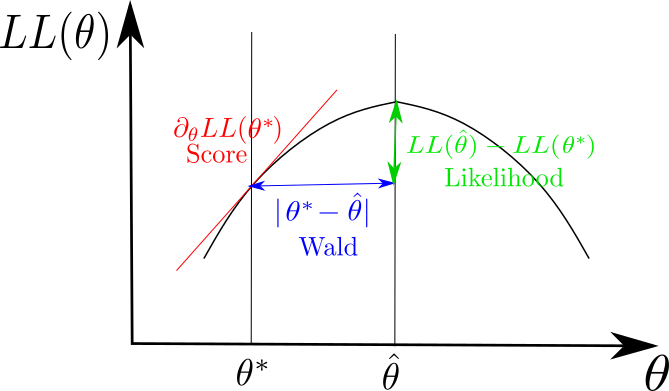
\includegraphics[width=3.2in]{conventions/classic-trio.png}
\caption{For $n=1$ and $\theta\in\RR$,
this figure shows the geometrical significance of
certain
quantities that
characterize the
3 classic test statistics
(Likelihood, Score, Wald)
for hypothesis testing.}
\label{fig-classic-trio}
\end{figure}

Henceforth in this section,
we will
occasionally  use the
Einstein summation
convention; i.e., implicit sum over
repeated indices.

Three classic test statistics
are (See Fig.\ref{fig-classic-trio}):

\begin{enumerate}

\item
{\bf Likelihood Ratio test statistic}
(Ref.\cite{wiki-Li-test}.)

\beq
\lam_{Li}=
2\ln\left[
\frac{L(\hat{\theta})}
{L(\theta^*)}
\right]=
2[LL(\hat{\theta})-LL(\theta^*)]
\eeq

\item
{\bf Score (a.k.a.
Lagrange multiplier) test statistic}
(Ref.\cite{wiki-Sc-test}.)

\beqa
\lam_{Sc}&=&
\partial_{\theta_i} LL(\theta^*)
\left[
FI(\theta^*)^{-1}\right]_{i,j}
\partial_{\theta_j} LL(\theta^*)
\\
&=&
\frac{[\partial_\theta LL(\theta^*)]^2}
{FI(\theta^*)}\quad \text{if $n=1$}
\eeqa
Doesn't depend on $\hat{\theta}$.

\item
{\bf Wald test statistic}
(Ref.\cite{wiki-Wa-test}.)


\beqa
\lam_{Wa}&=&
(\hat{\theta}-\theta^*)_i
\left[
\av{\hat{\rvtheta},\hat{\rvtheta}^T}^{-1}
\right]_{i,j}
(\hat{\theta}-\theta^*)_j
\label{eq-wald-stat}
\\
&=&
\frac{(\theta^*-\hat{\theta})^2}
{\av{\hat{\theta},\hat{\theta}}}
\quad\text{if $n=1$}
\eeqa

More generally,
one can replace $\theta^*\rarrow R\theta^*$
and  $\hat{\theta}\rarrow R\hat{\theta}$
in Eq.(\ref{eq-wald-stat}),
where $\theta^*$ and
$\hat{\theta}$ are $n$ dimensional
column vectors, and
$R\in\RR^{\nu\times n}$.
The null and alternative hypotheses become:
$H_0: R\theta=R\theta^*$
and $H_1: R\theta\neq R\theta^*$.
Note that
$\nu$
is the number of
constraints imposed by the
null hypothesis. $R$ is called a
reparametrization of $\theta$.
The Wald test is not
reparametrization
invariant (i.e., $R$
invariant), but the Likelihood Ratio test is.

\end{enumerate}

Note that
if $LL(\theta)$
is given by Eq.(\ref{eq-normal-ll}),
then
$\av{\hat{\rvtheta},\hat{\rvtheta}}
=
\s^2=\frac{1}{FI(\theta)}
$. Hence,

\beq
\lam_{Li}=\lam_{Sc}=\lam_{Wa}=
\frac{(\hat{\theta}-\theta^*)^2}{\s^2}
\eeq

Many
other commonly used test statistics
(or their squares)
are special cases of one
of the 3 classic test statistics.
For example, the z-statistic
used with normal
distributions,
the t-statistic
used with the
Student t-distribution,
the F-statistic used in linear regression,
the chi-squared statistic used
to do Pearson's chi-squared test.

{\bf Asymptotic Behavior}

If the data
$\vec{x}$ is i.i.d.,

\beq
P(\vec{x}|\theta)=
\prod_{\s=0}^{nsam-1} P(x^\s|\theta)
\;
\eeq
Hence, as $nsam\rarrow \infty$,

\beqa
LL(\theta)
&=&
\ln P(\vec{x}|\theta)
\\
&=&\sum_\s \ln
P(x^\s|\theta)
\\
&\rarrow&
nsam \sum_x P(x|\theta)\ln  P(x|\theta)
\\
&=&
-nsam \; H(\rvx|\theta)
\eeqa
Thus, {\it maximizing} the log likehood
$LL(\theta)$
and {\it minimizing} the entropy
$H(\rvx|\theta)$
give the same estimate $\hat{\theta}$.

When the
data is i.i.d. and
$nsam\rarrow \infty$,
it is also possible to
prove that
the 3 test statistics
defined above all tend to
the same
probability  distribution, namely
$\calx^2(\theta^*; \nu)$,
the chi-square distribution
with $\nu$ degrees of freedom,
where $\theta\in \RR^n$, $R\in \RR^
{\nu\times n}$, and $\nu=n$ if $R=1$.

\section{Error Bars}
Never report measurements without error bars!!

Assume a distribution
with mean $\mu$ and
standard deviation $\s$
for a subpopulation with $n$
samples.

$SE=\frac{\s}{\sqrt{n}}$
is called the {\bf standard error}.


Some popular types of error bars:


\begin{itemize}
\item{\bf Box and Whiskers plot (a.k.a. Boxplot)}

See Fig.\ref{fig-boxplot}.
$IQR$ stands for {\bf
Intermediate Quantile Range}.
Sometimes, the endpoints of the
error bars are taken to be the minimum and maximum samples
instead of $Q_1- 1.5 *IQR$ and $Q_3+ 1.5 *IQR$.
The points that fall
in the intervals $[\min,Q_1- 1.5* IQR]$
and $[Q_3+ 1.5 *IQR, \max]$
are
called {\bf outliers}.
\begin{figure}[h!]
\centering
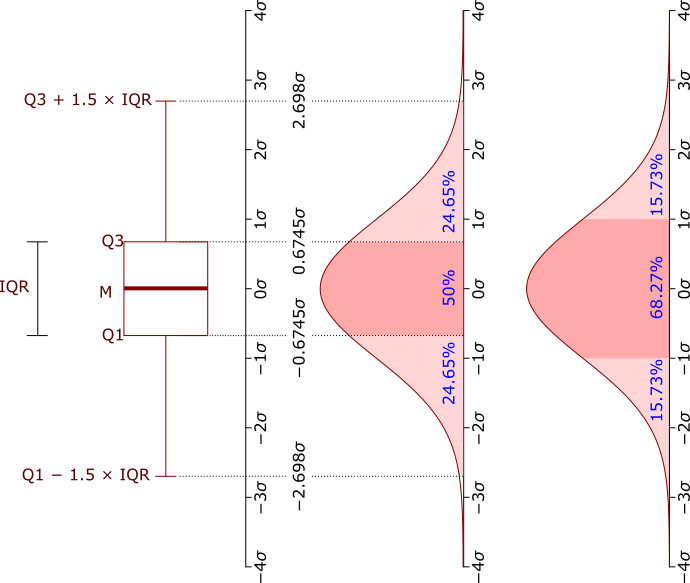
\includegraphics[width=3.3in]
{conventions/Boxplot.png}
\caption{Boxplot plot for Normal
distribution $\caln(\mu=0,\s)$.
$Q_1$ and $Q_3$ are the first and third
quantiles, and $M$ is the median (i.e., half-way point).
For a non-normal skewed
distribution, $Q_1$ and $Q_3$
are not equidistant from the median, and the
median is not exactly equal to the mean. }
 \label{fig-boxplot}
\end{figure}



\item{\bf Standard Deviation}

Error bar endpoints are located one standard deviation
away from the mean.
\beq
\mu-\s< \mu < \mu+\s
\eeq

\item{\bf Confidence Interval}

\beq
\mu-|z^*|SE <\mu < \mu+|z^*|SE
\label{eq-conf-int}
\eeq

$|z^*|=1.96$ for a confidence level of $95\%$.

The origin of Eq.(\ref{eq-conf-int})
is explained in the next section entitled ``Confidence Intervals".
Confidence intervals are
derived from the Gaussian in Fig.\ref{fig-conf-int},
which should not be confused with the
Gaussian of Fig.\ref{fig-boxplot}.
They are different!

\end{itemize}
\section{Confidence Intervals}

Normal distribution
with mean $\mu$
and standard deviation $\sigma$:

\beq
\caln(x;\mu, \s^2)=
\frac{1}{\s\sqrt{2\pi}}
e^{- \frac{(x-\mu)^2}{2\sigma^2}}
\;.
\eeq

Standard Normal Distribution (SND):
\beq
P(z)=\caln(z;0,1)
\eeq
Cumulative distribution for $P(z)$:

\beq
\Phi(z)=\int_{-\infty}^z dz'\;P(z')
\;.
\eeq

\begin{figure}[h!]
\centering
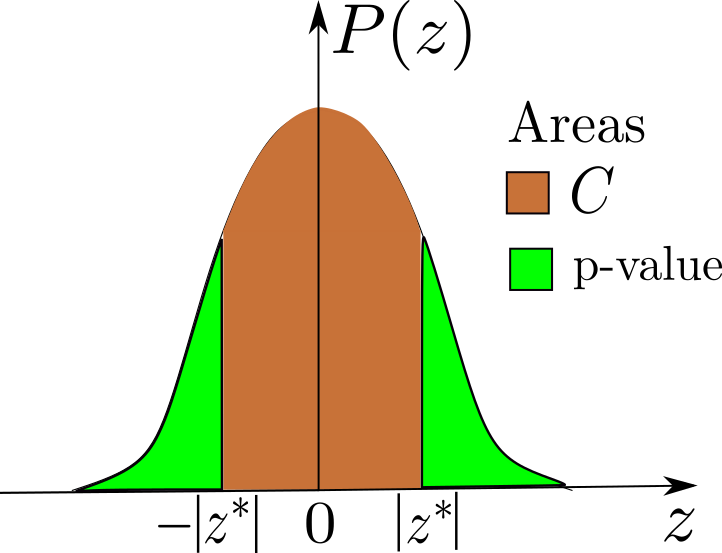
\includegraphics[width=2in]
{conventions/conf-int.png}
\caption{
Interpretation
of confidence level $C$
and p-value as areas under curve of the
Standard Normal Distribution (SND).}
\label{fig-conf-int}
\end{figure}

{\bf Confidence Level} $C$
and corresponding {\bf $|z^*|$ value}
(see Fig.\ref{fig-conf-int}):

\beq
C=\int_{-|z^*|}^{|z^*|} dz\;P(z) =
\Phi(|z^*|)-\Phi(-|z^*|)
=
2\left(\Phi(|z^*|)-\frac{1}{2}\right)
\label{eq-conf-level1}
\eeq
Equivalent definition:

\beq
C=P\left(
\underbrace{
\frac{|\rvx-\mu|}{\frac{\sigma}{\sqrt{n}}}
}_{|\rvz|}
<|z^*|\right)
\label{eq-conf-level2}
\eeq
For $C=95\%$,
$|z^*|=1.960\approx 2$.
For $C=99\%$, $|z^*|=2.576$.

Area of each tail
in Fig.\ref{fig-conf-int} is
usually called $\alpha$,
and the area of both tails is called
the {\bf p-value}:
\beq
C+\underbrace{2\alpha}_{p-value}=1
\;.
\eeq

Estimators\footnote{Don't
confuse the sample index $\s$
with the standard deviation $\s$.} of
mean $\mu$  and
standard deviation $\sigma$
from measurements $x^\s$
of a sub-population $\Sigma_1$ of
size $n=|\Sigma_1|$:
\beq
\hat{\mu}=\ol{x}=\frac{1}{n}\sum_{\s \in\Sigma_1} x^\s
\eeq

\beq
\hat{\s}^2=
\frac{1}{n-1}
\sum_{\s\in \Sigma_1} (x^\s-\ol{x})^2
\eeq


We get
from Eq.(\ref{eq-conf-level2}),
the {\bf Error bars (a.k.a. confidence intervals)}
and
{\bf Error $E$ (a.k.a. margin of error)}:



\beq
\text{ estimate of $x$
with error bars} =
\ol{x} \pm
\underbrace{
|z^*| \frac{\hat{\s}}{\sqrt{n}}}_{E}
\label{eq-err-bars}
\eeq

\beq
n= \left(
\frac{|z^*|\hat{\s}}{E}
\right)^2
\eeq

So far, we have assumed
that the sub-population (a.k.a. sample
population)
is normally distributed.
This might be false
for several reasons.
Some red flags: (1)
$n$ is too small (according to
a rule of thumb derived from
Central Limit Theorem, $n$
should be larger than 30
to insure a Normal Distribution).
(2) Sub-population not truly random
(i.i.d.)
because was taken
without replacement.
In many cases,
especially
when $n<30$,
the Student's t-distribution
models the sub-population statistics
much
better than the Normal distribution.


The {\rm Student's t-distribution } ${\rm Stud}(t;
\nu=n-1)$,
depends
on a parameter $\nu$
called the
number of
degrees of freedom.
In the case being considered here,
$\nu$ equals the
sub-population size $n$
minus one.
When fitting
the data with
Stud(), variable
$t$ replaces
variable $z$,
and ${\rm Stud}(t; \nu=n-1)$
replaces the Standard Normal distribution (SND)
$\caln(z; \mu=0, \sigma=1)$.
Stud() is symmetric about
the origin like SND,
but its tails
are fatter.
When fitting the data with Stud(),
the $|z^*|$
value is replaced
by a $|t^*|$ value.
Eq.(\ref{eq-conf-level1})
is replaced by


\beq
C=\int_{-|t^*|}^{|t^*|} dt\;{\rm Stud}(t) =
\Phi_S(|t^*|)-\Phi_S(-|t^*|)
=
2\left(\Phi_S(|t^*|)-\frac{1}{2}\right)
\label{eq-conf-level1-stu}
\;,
\eeq
where $\Phi_S()$
is the cumulative
distribution for  Stud().
Also, Eq.(\ref{eq-err-bars})
is replaced  by

\beq
\text{estimate of $x$
with error bars} =
\ol{x} \pm
\underbrace{
|t^*| \frac{\hat{\s}}{\sqrt{n}}}_{E}
\;.
\eeq
Tables of $|t^*|(C,\nu=n-1)$
are available. Note
that $|t^*|$
depends on both $C$ and $\nu$,
whereas $|z^*|(C)$
depends only on $C$.

\section{p-value, general definition}


Given a parameter $\theta$, call
$\theta=\theta_0$ (or  $\theta<\theta_0$ or $\theta>\theta_0$) the
{\bf null hypothesis} $h_0$,
and call the negation of $h_0$ the {\bf alternative hypothesis} $h_1$.
Assume we
are given data $\vec{x}=\{x^\s|\s\in \Sigma\}$. Assume
also that we are given
distributions $P(\rvx=x|h)$ for $h\in \{h_0, h_1\}$,
and $P(\rvx=x)$. Now let

\beq
P(\vec{x}|h)=\prod_\s P(\rvx=x^\s|h)
\eeq


\beq
P(\vec{x})=\prod_\s P(\rvx=x^\s)
\eeq
(so the $x^\s$ are i.i.d.).

A Bayesian would assume that there
is a prior $P(h)$, and use it to
calculate
$P(h|\vec{x})=\frac{P(\vec{x}|h) P(h)}{P(\vec{x})}$.
$P(\rvh\neq h_0|\vec{x})$
is the probability that the null hypothesis is false.
A p-value is a monotonically increasing function of
$P(\rvh\neq h_0|\vec{x})$,
so Bayesians have no trouble saying
that  {\color{red} a p-value is
a measure of
$P(\rvh\neq h_0|\vec{x})$, i.e.,
a measure of the probability that
the null-hypothesis is false}.

Frequentists, on the other hand,
believe that $h$
is a ``parameter", not a random variable,
so  $P(\rvh\neq h_0|\vec{x})$
is undefined.
Next, we explain the correct
way of thinking about p-values, according to
Frequentists.
p-values were invented by Frequentists,
so it's worth hearing what they have to say
about them.
The Frequentist definition is not against Bayesianism,
and Bayesians, unlike Frequentists,
 don't accuse Frequentists of
having a sinfully incorrect
 definition of p-values. A Bayesian would just say:
our definition of p-values (shown
in red above) is not incorrect,
but the Frequentist definition is more precise than ours,
and doesn't assume a particular form for a prior.
We welcome it.

Call
the random variable
$\rvt$ the {\bf test statistic} and the function
$OTS(\vecx)$ the {\bf observed test statistic}.
$OTS(\vecx)$ is designed so that
it becomes 0 when $h_0$
is exactly satisfied,
and its magnitude grows monotonically as $h_0$
becomes less well satisfied.
Frequentists define the {\bf p-value} $p$ as

\beq
p=
\left\{
\begin{array}{ll}
P(\rvt \geq OTS(\vecx)|h_0)&\text{right-sided-tail,
if $h_0$ is $\theta<\theta_0$}
 \\
 P(\rvt\leq OTS(\vecx)|h_0)&\text{left-sided-tail,
 if $h_0$ is $\theta>\theta_0$}
 \\
 P(|\rvt| > |OTS(\vecx)|\;|h_0)&\text{double-sided-tail,
 if $h_0$ is $\theta=\theta_0$}
\end{array}
\right.
\eeq
Thus, for a Frequentist,
{\color{red} a p-value is a probabilistic
measure of the size of the region
where the $h_0$ hypothesis is
extremely violated}.
If that region is large,
then the region where
the $h_0$ hypothesis
is approximately satisfied is small,
which means the $h_0$
hypothesis
is approximately satisfied.
The smaller the p-value, the
less likely it is that the $h_0$
hypothesis is true,
just like the Bayesian definition
says.
Note that the p-value
is a probability so it ranges in
value from 0 to 1.

Suppose we are given a subpopulation with $n$ samples,
 mean $\ol{x}$ and variance $\hat{\s}$.
 Let $\theta_0=\mu_0$.
 For the z-test and the t-test,
we define

\beq
\rvt=\rvz=
\frac{\rvx-\mu}{\frac{\hat{\s}}{\sqrt{n}}}, \quad
OTS(\vecx)=z^*
\;,
\eeq
where
the {\bf z-score} $z^*$ is defined by


\beq
z^*=\frac{\ol{x}-\mu_0}{\frac{\hat{\s}}{\sqrt{n}}}
\;.
\eeq
For a {\bf z-test},

\begin{subequations}
\beqa
P(\rvz\geq z^*|h_0)=\Phi(z^*)
&\quad&\text{if $h_0$ is $\mu<\mu_0$}
\\
P(\rvz\leq z^*|h_0)=1-\Phi(z^*)=\Phi(-z^*)
&\quad&\text{if $h_0$ is $\mu>\mu_0$}
\\
P(|\rvz|\geq |z^*|\;|h_0)=2\Phi(-|z^*|)
&\quad&\text{if $h_0$ is $\mu=\mu_0$}
\label{eq-double-tail}
\eeqa
\end{subequations}
where $\Phi(x)$ is the cumulative distribution
for the Standard Normal Distribution
$\caln(x;\mu=0, \s=0)$.
For a {\bf t-test}, $\Phi()$ is replaced
by $\Phi_S()$, where  $\Phi_S()$ is
the cumulative distribution
for the Student t-distribution ${\rm Stud}(x; \nu=n-1)$.
Note that Eq.(\ref{eq-double-tail})
agrees with
Eq.(\ref{eq-conf-level2}).

\section{Short Summary of
Boolean Algebra}
See Ref.\cite{wiki-bool} for more info
about this topic.

Suppose $x, y, z\in \bool$. Define

\beq
x\text{ or }y=x\V y= x+y-xy
\;,
\eeq

\beq
x \text{ and }y=x\A y= xy
\;,
\eeq
and

\beq
\text{not }x=\ol{x}=1-x
\;,
\eeq
where we are using
normal addition and multiplication
on the right hand sides.\footnote{Note the
difference between $\V$ and modulus
2 addition $\oplus$.
For $\oplus$ (a.k.a. XOR): $x\oplus y=x+y-2xy$.}



\begin{table}[h!]
\centering
\begin{tabular}{|
>{\columncolor[HTML]{ECF4FF}}l |l|}
\hline
Associativity & \begin{tabular}[c]{@{}l@{}}$x \V (y \V z)=(x \V y) \V z$\\ $x \A (y \A z)=(x \A y) \A z$\end{tabular} \\ \hline
Commutativity & \begin{tabular}[c]{@{}l@{}}$x \V y=y \V x$\\ $x \A y=y \A x$\end{tabular} \\ \hline
Distributivity & \begin{tabular}[c]{@{}l@{}}$x \A (y \V z)=(x \A y) \V (x \A z)$\\ $x \V (y \A z)=(x \V y) \A (x \V z)$\end{tabular} \\ \hline
Identity & \begin{tabular}[c]{@{}l@{}}$x \V 0=x$\\ $x \A 1=x$\end{tabular} \\ \hline
Annihilator & \begin{tabular}[c]{@{}l@{}}$x \A 0=0$\\ $x \V 1= 1$\end{tabular} \\ \hline
Idempotence & \begin{tabular}[c]{@{}l@{}}$x \V x= x$\\ $x \A x= x$\end{tabular} \\ \hline
Absorption & \begin{tabular}[c]{@{}l@{}}$x \A (x \V y)= x$\\ $x \V (x \A y)= x$\end{tabular} \\ \hline
Complementation & \begin{tabular}[c]{@{}l@{}}$x \A \ol{x} = 0$\\ $x \V \ol{x}   = 1$\end{tabular} \\ \hline
Double negation & $\ol{(\ol{x})} = x$ \\ \hline
De Morgan Laws & \begin{tabular}[c]{@{}l@{}}$\ol{x} \A \ol{y} =\ol{(x \V y)}$\\ $\ol{x} \V \ol{y} = \ol{(x \A y)}$\end{tabular} \\ \hline
\end{tabular}
\caption{Boolean Algebra Identities}
\label{tab-bool-alg}
\end{table}

Actually, since
$x\A y=xy$, we can omit writing
the symbol $\A$. The symbol
$\A$ is useful to
exhibit the symmetry
of the identities, and
to remark
about
the analogous identities
for sets, where
$\A$ becomes intersection $\cap$
and $\V$ becomes union $\cup$. However,
for practical calculations,
$\A$ is an unnecessary nuisance.

Since $x\in \bool$,
\beq
P(\ol{x})=1-P(x)
\;.
\eeq

Clearly, from analyzing
the simple event space $(x,y)\in \bool^2$,
\beq
P(x\V y)= P(x) + P(y) - P(x\A y)
\;.
\eeq
